\chapter{Governo eletrônico e digital no Brasil}

\cite{tavares2022governo} ressalta que a Constituição Federal de 1988 fixou a cidadania como fundamento da República, tendo a participação e o controle papéis essenciais ao bom funcionamento do Estado, da Democracia e da Administração Pública, a partir da concepção de cidadania e democracia participativa.

Além disso, \cite{tavares2022governo} argumenta que o controle social possui estreita ligação com as políticas públicas, pois, a partir do seu exercício, em todas as etapas do ciclo, desde a formulação até a avaliação, confere-se maior legitimidade e eficiência aos resultados dos objetivos, metas e diretrizes fixadas pelos planos, programas e ações dentro do conjunto de políticas públicas.

Adicionalmente, \cite{tavares2022governo} afirma que as políticas públicas são a forma como se resolve os problemas da sociedade e o controle social é a forma como o cidadão interage, fiscaliza e questiona as soluções definidas para esses problemas. 

Como consequência, \cite{Guimaraes2005} argumenta que o governo eletrônico foi visto como uma oportunidade de incrementar a participação da sociedade na gestão pública, especialmente quanto à formulação, ao acompanhamento e à avaliação das políticas públicas, visando ao incremento da cidadania e da democracia. 

\cite{rover2009introduccao} argumenta que a interação entre as novas tecnologias, a sociedade e o Poder Público emoldura um momento único do qual emergem, simultaneamente, desafios enormes e vantagens sociais incríveis. Neste contexto, o aparecimento do governo eletrônico é uma decorrência das velhas e novas demandas da sociedade.

Para \cite{rover2009introduccao}, governo eletrônico é uma infra-estrutura única de comunicação compartilhada por diferentes órgãos públicos a partir da qual a TIC é usada de forma intensiva para melhorar a gestão pública e o atendimento ao cidadão.

Adicionalmente, como é entendido por \cite{rover2009introduccao}, o objetivo do governo eletrônico é colocar o governo ao alcance de todos, ampliando a transparências das suas ações e incrementando a participação cidadã, almejando a universalização de serviços.

\cite{singh2007country} projeta que a maturidade do governo eletrôncio pode ser considerada razoavelmente dependente de como está o estado da infraestrutura de TIC, em razão da sua capacidade de limitar o acesso aos serviços públicos digitais. 

Para \cite{singh2007country}, países com PIB per capita altos estão em melhor posição de dispor de infraestruturas difundidas, alta qualidade e físicas de TIC. Com altos níveis de acesso às TIC, os cidadãos tem uma tendência maior de usar serviços públicos digitais.

Quando os cidadãos passam a adotar os serviços públicos digitais, segundo \cite{singh2007country}, facilita ao poder público a transação completa dos serviços públicos presenciais para os digitais. A referida mudança pode ajudar na economia de recursos públicos, definindo um círculo virtuoso que justifica os investimentos em governo eletrônico.

Diversos autores destacam o impacto positivo do governo eletrônico na sociedade. Suas conclusões estão presentes na figura \ref{fig:tabela_beneficios_egov}.

\begin{figure}[H]
	\centering
	\caption{Revisão da literatura dos benefícios do governo
eletrônico}
	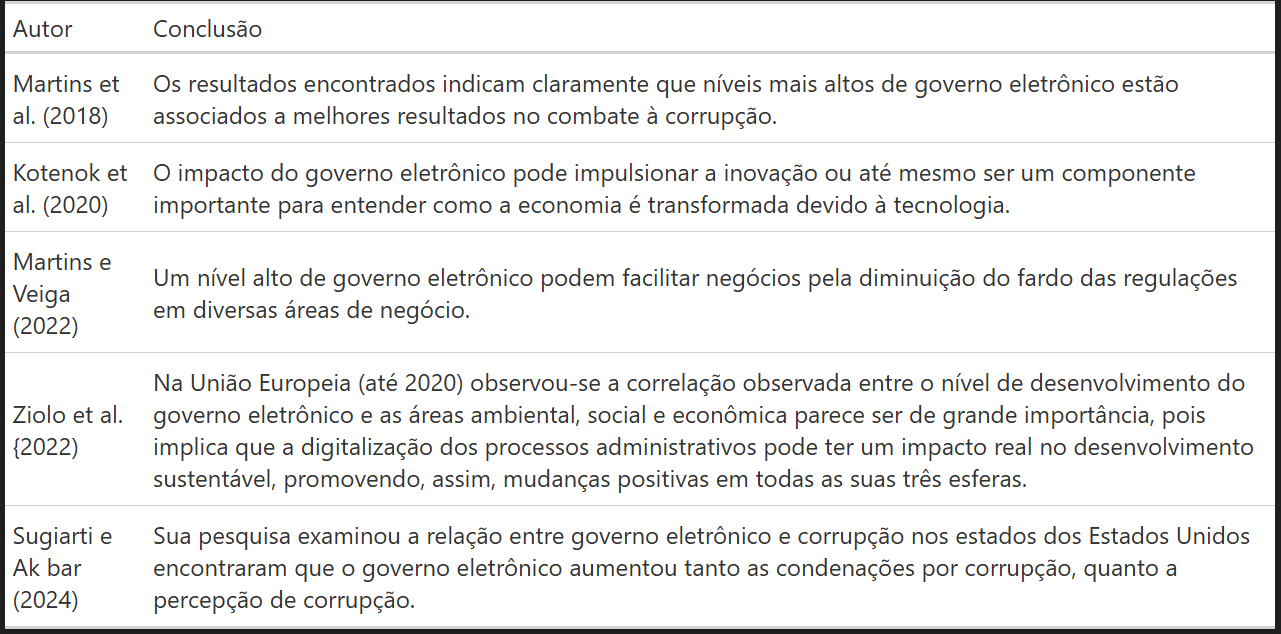
\includegraphics[width=1\linewidth]{figuras/tabela_beneficios_egov.png}
	\label{fig:tabela_beneficios_egov}
	\footnotesize{Fonte: elaboração própria.}
\end{figure}

Como exposto pela figura \ref{fig:tabela_beneficios_egov}, percebe-se quão benéfico é o governo eletrônico tanto para os governos, quanto para o povo. Dentre os benefícios, destaca-se a participação social. 

Contudo, para \cite{de2020governo} o foco das políticas de governo eletrônico, em geral, permanece o mesmo: aprimorar processos internos de  trabalho, sem alterações significativas na cultura e na lógica burocráticas sobre as quais se estruturam as relações que se estabelecem entre a administração pública e os cidadãos.

Assim, para \cite{cristovam2020governo} a Administração Pública brasileira tem usado as TIC no incremento de suas rotinas burocráticas. Há, ainda, o crescente uso dessas tecnologias na promoção do acesso à informação aos cidadãos. Mas ambos são usos na esteira do dito Governo eletrônico.

Consequentemente, conforme \cite{cristovam2020governo}, para se distanciar do governo eletrônico e poder implementar o governo digital, pois não se deve almeja somente o emprego incremental de TICs e a viabilização do acesso à informação, mas vai além, corporificando direitos sociais por intermédio do espaço digital.

Nesse sentido, quando \cite{cristovam2020governo} afirma que as TIC podem contribuir para a inovação e o fomento da prestação de serviços públicos adequados e atuais para todos os cidadãos, comportando as dimensões democrática e social impostas pela ordem jurídica constitucional vigente, há convergência com a ideia expressa por \cite{kotenok2020government} na tabela \ref{fig:tabela_beneficios_egov}.

No dado contexto, \cite{alenezi2022understanding} afirma que sua pesquisa destaca que um ambiente efetivo e favorável, força de trabalho qualificada, liderança, políticas públicas e regulações são os fatores-chave do sucesso que podem encorajar e facilitar a rápida adaptação da transformação digital nas organizações do setor público.

Como expressado nos parágrafos anteriores, com as condições favoráveis, a transformação digital pode se tornar paupável, executável e planejável. Segundo \cite{mitkiewicz2024transformacao}, a transformação digital pode ser entendida como o processo de utilização das tecnologias da informação e comunicação para gerar soluções visando resolver de forma inovadora e em larga escala os problemas do mundo.

De forma complementar, \cite{alenezi2022understanding} afirma que a transformação digital no governo ou no setor público refere-se ao engajamento diferente e inovador e o trabalho com as partes interessadas, desenvolvendo frameworks para os mecanismos de entrega de serviços eficientes e formação de novos relacionamentos.

No contexto dos parágrafos anteriores, surgem os governos digitais em substituição aos governos eletrônicos. \cite{veiga2016digital} afirma que, diferentemente do governo eletrônico, o governo digital não é apenas sobre tecnologia, é sobre uma operação multifacetada  que requer uma abordagem multidisciplinar e disciplina científica. 

\cite{bounabat2017government} complementa a ideia anterior. O auto cita que o governo digital baseia-se na divulgação aberta e sem precedentes de informações governamentais, aliada à troca em grande volume de informações altamente sensíveis e também pessoais entre agências governamentais e seus clientes. 

O governo digital traz diversos benefícios, além dos benefícios do governo eletrônico. \cite{martins2018war} argumenta que as ferramentas de governo digital promovem transparência, responsabilização e acesso melhorado à informação.

Outra vantagem é mencionada por \cite{veiga2016digital}. O autor afirma que o uso de governo digital e serviços públicos online têm um grande potencial de reduzir o fardo administrativo, bem como, promover inovação e crescimento econômico. Além de contribuir com a diminuição das atividades da economia informal, aumentando a quantidade de pessoas que pagam impostos e reduzing a corrupção.

\section{Entendendo o governo eletrônico no Brasil sob a ótica da pesquisa TIC Domicílios 2024 da Cetic.BR}

Como forma de entender o uso do governo eletrônico no Brasil, optou-se por \cite{tic_domicilios_2024}, devido ao seu objetivo de mapear o acesso às TIC nos domicílios urbanos e rurais do país e as suas formas de uso por indivíduos de 10 anos de idade ou mais. E ao fato de que o uso de governo eletrônico ser uma das suas áreas de investigação.

Em razão da continuidade das pesquisa \href{https://cetic.br/pt/pesquisa/domicilios/}{TIC Domicílios} desde 2005, escolheu-se o último de pesquisa (\textbf{2024}) da Cetic.BR. O tópico G foi o escolhido. Dele serão usados todos os seus indicadores (\href{https://cetic.br/pt/tics/domicilios/2024/individuos/G1/}{G1}, \href{https://cetic.br/pt/tics/domicilios/2024/individuos/G2/}{G2}, \href{https://cetic.br/pt/tics/domicilios/2024/individuos/G2A/}{G2A}, \href{https://cetic.br/pt/tics/domicilios/2024/individuos/G3/}{G3}). O primeiro, o G1, revelou o percentual de uso de governo eletrônico por indivíduos, cujo resultado está presente na figura \ref{fig:mapa_coropletico_tic_domicilio_g1}.

\begin{figure}[H]
	\centering
	\caption{Indicador G1: Uso de governo eletrônico por região do Brasil}
	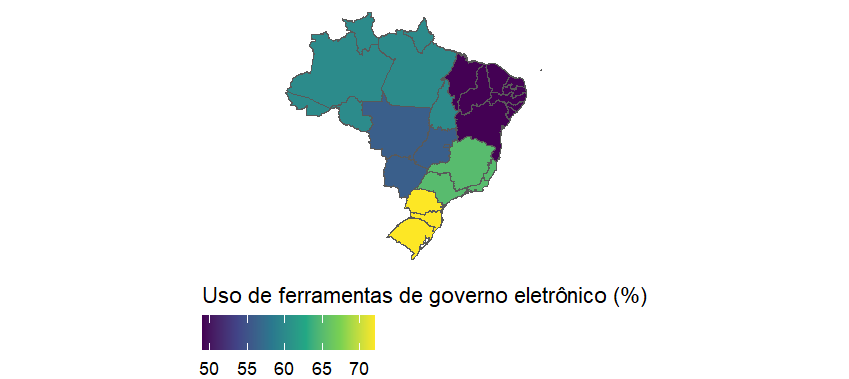
\includegraphics[width=1\linewidth]{figuras/mapa_coropletico_tic_domicilios_2024_g1}
	\label{fig:mapa_coropletico_tic_domicilio_g1}
	\footnotesize{Fonte: \cite{tic_domicilios_2024_g1}.}
\end{figure}

A figura \ref{fig:mapa_coropletico_tic_domicilio_g1} representa os resultados do indicador G1. As regiões Sul e Sudeste são as regiões que mais usam o governo eletrônico, seguidas das regiões Centro-Oeste e Norte. Por último, está o Nordeste.

O indicador G2 complementa o G1 ao especificar quais grupos de funções de governo eletrônico foram os mais usados. O indicador G2 tem os seguintes critérios:

\begin{figure}[H]
	\centering
	\caption{Critérios do indicador G2}
	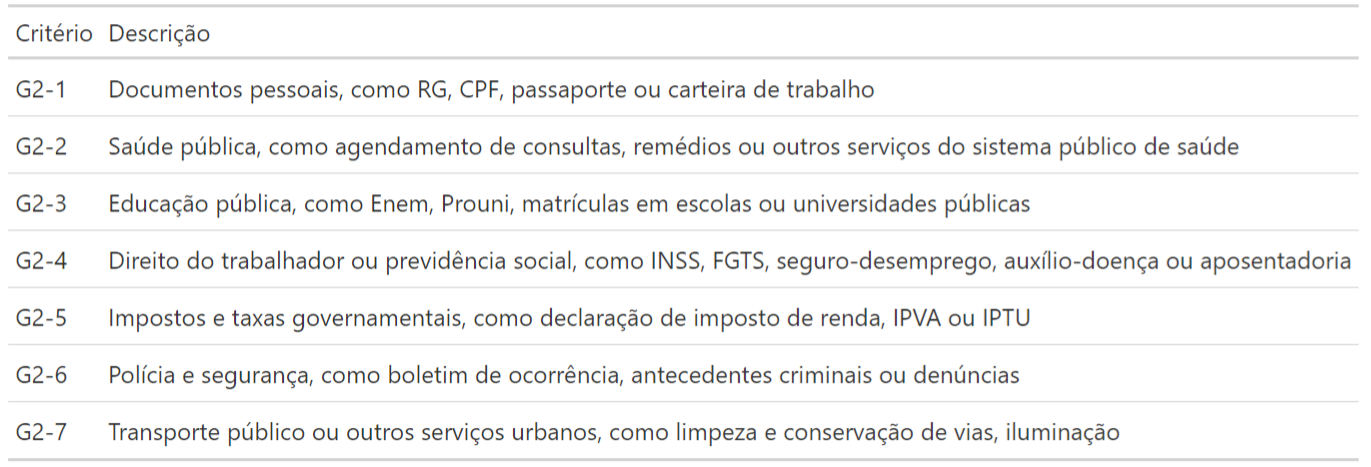
\includegraphics[width=1\linewidth]{figuras/tabela_tic_domicilios_2024_criterios_g2.png}
	\label{fig:tabela_tic_domicilios_2024_criterios_g2}
	\footnotesize{Fonte: \cite{tic_domicilios_2024_g2}.}
\end{figure}

As figuras seguintes detalham como cada critério é usado por região.

\begin{figure}[H]
	\centering
	\caption{Indicador G2: critérios 1 e 2}
	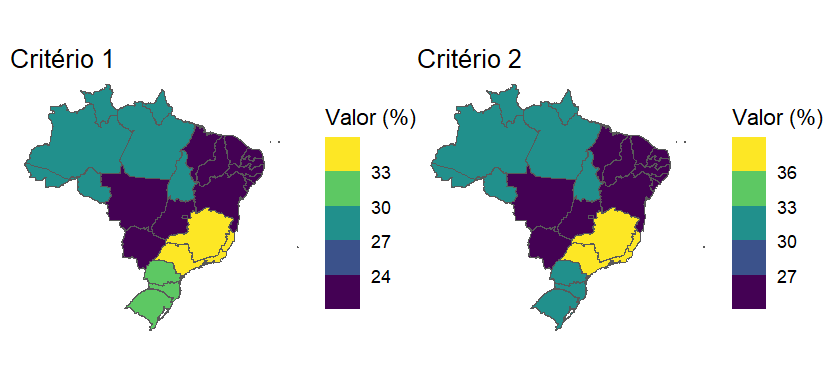
\includegraphics[width=1\linewidth]{figuras/mapa_coropletico_tic_domicilios_2024_g2_1_2.png}
	\label{fig:mapa_coropletico_tic_domicilios_2024_g2_1_2}
	\footnotesize{Fonte: \cite{tic_domicilios_2024_g2}.}
\end{figure}

Quando se trata do indicador G2-1, as regiões que mais buscaram serviços públicos relativos a documentos pessoais, como RG, CPF, passaporte ou carteira de trabalho foram as Norte, Sudeste e Sul;

Quando se trata do indicador G2-2, apenas o Nordeste foi a região que menos uso serviços públicos relativos à saúde pública, como agendamento de consultas, remédios ou outros serviços do sistema público de saúde.

\begin{figure}[H]
	\centering
	\caption{Indicador G2: critérios 3 e 4}
	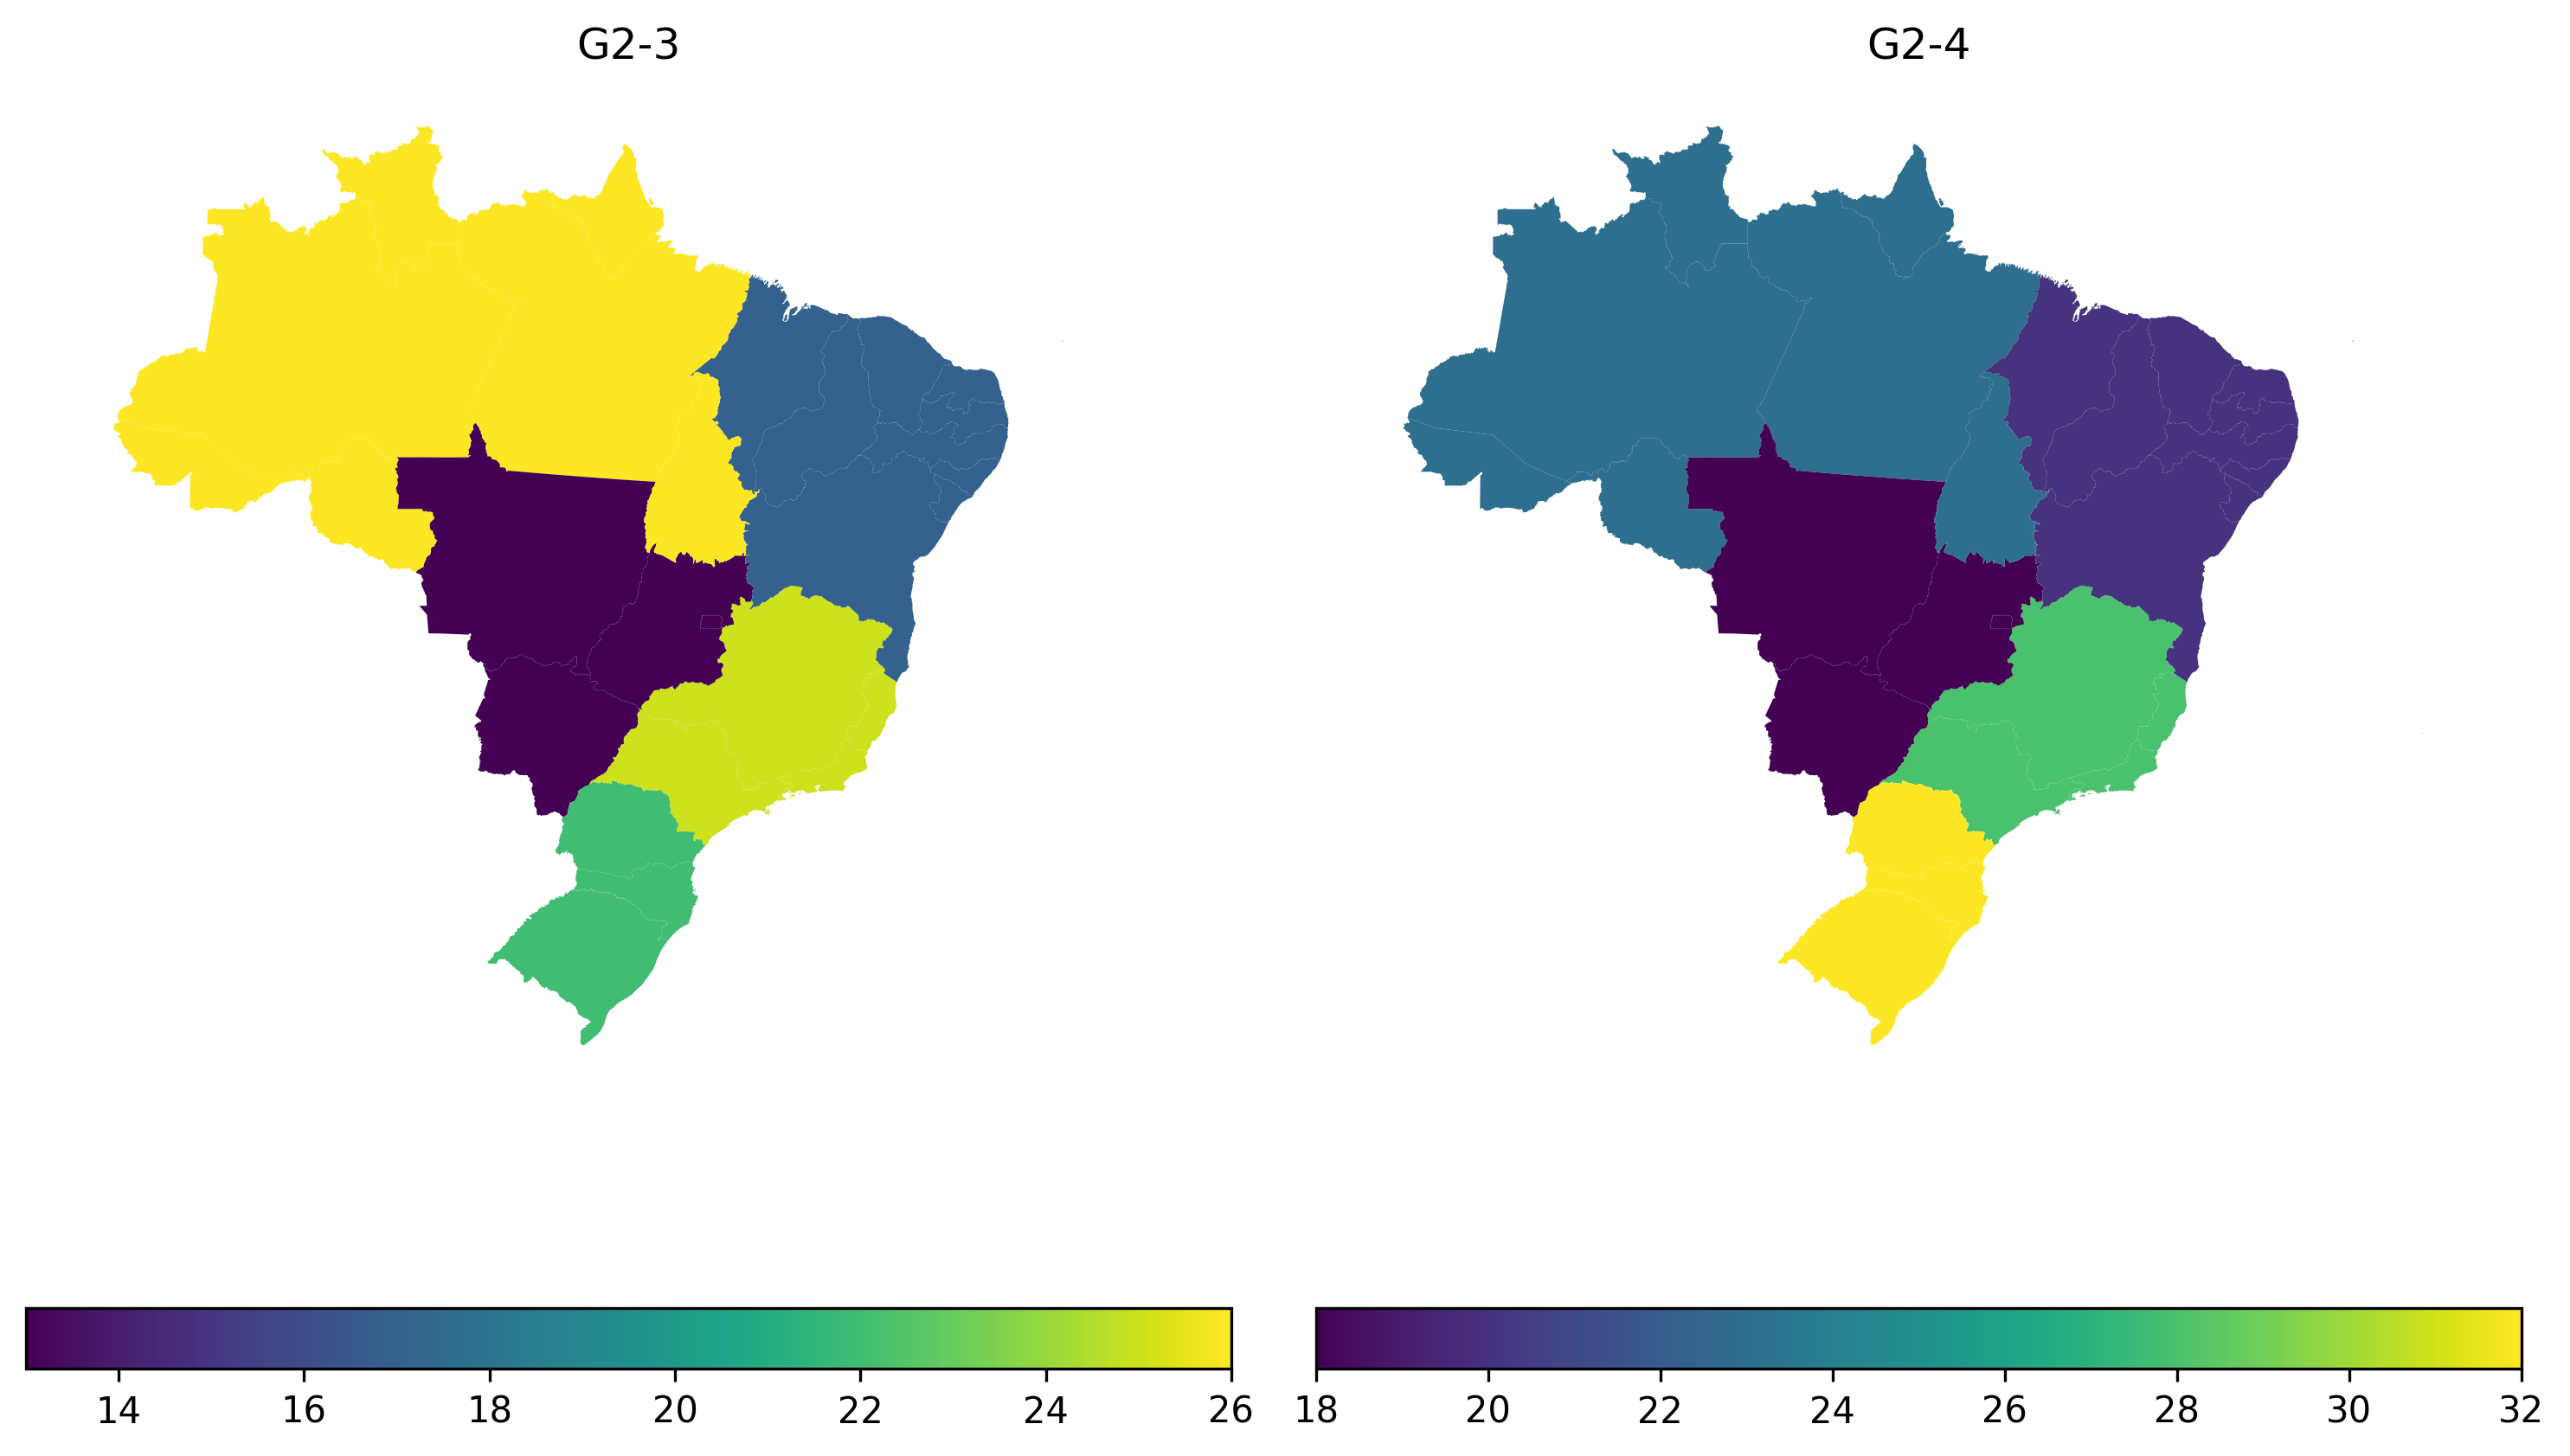
\includegraphics[width=1\linewidth]{figuras/mapa_coropletico_tic_domicilios_2024_g2_3_4.png}
	\label{fig:mapa_coropletico_tic_domicilios_2024_g2_3_4}
	\footnotesize{Fonte: \cite{tic_domicilios_2024_g2}.}
\end{figure}

Quando se trata do indicador G2-3, as regiões que mais usam serviços públicos relativos à educação pública, como Enem, Prouni, matrículas em escolas ou universidades públicas foram a Norte e a Sudeste.

Quando se trata do indicador G2-4, as regiões que mais usar serviços públicos relativos ao direito do trabalhador ou previdência social, como INSS, FGTS, seguro-desemprego, auxílio-doença ou aposentadoria foram as Sudeste e a Sul.

\begin{figure}[H]
	\centering
	\caption{Indicador G2: critérios 5 e 6}
	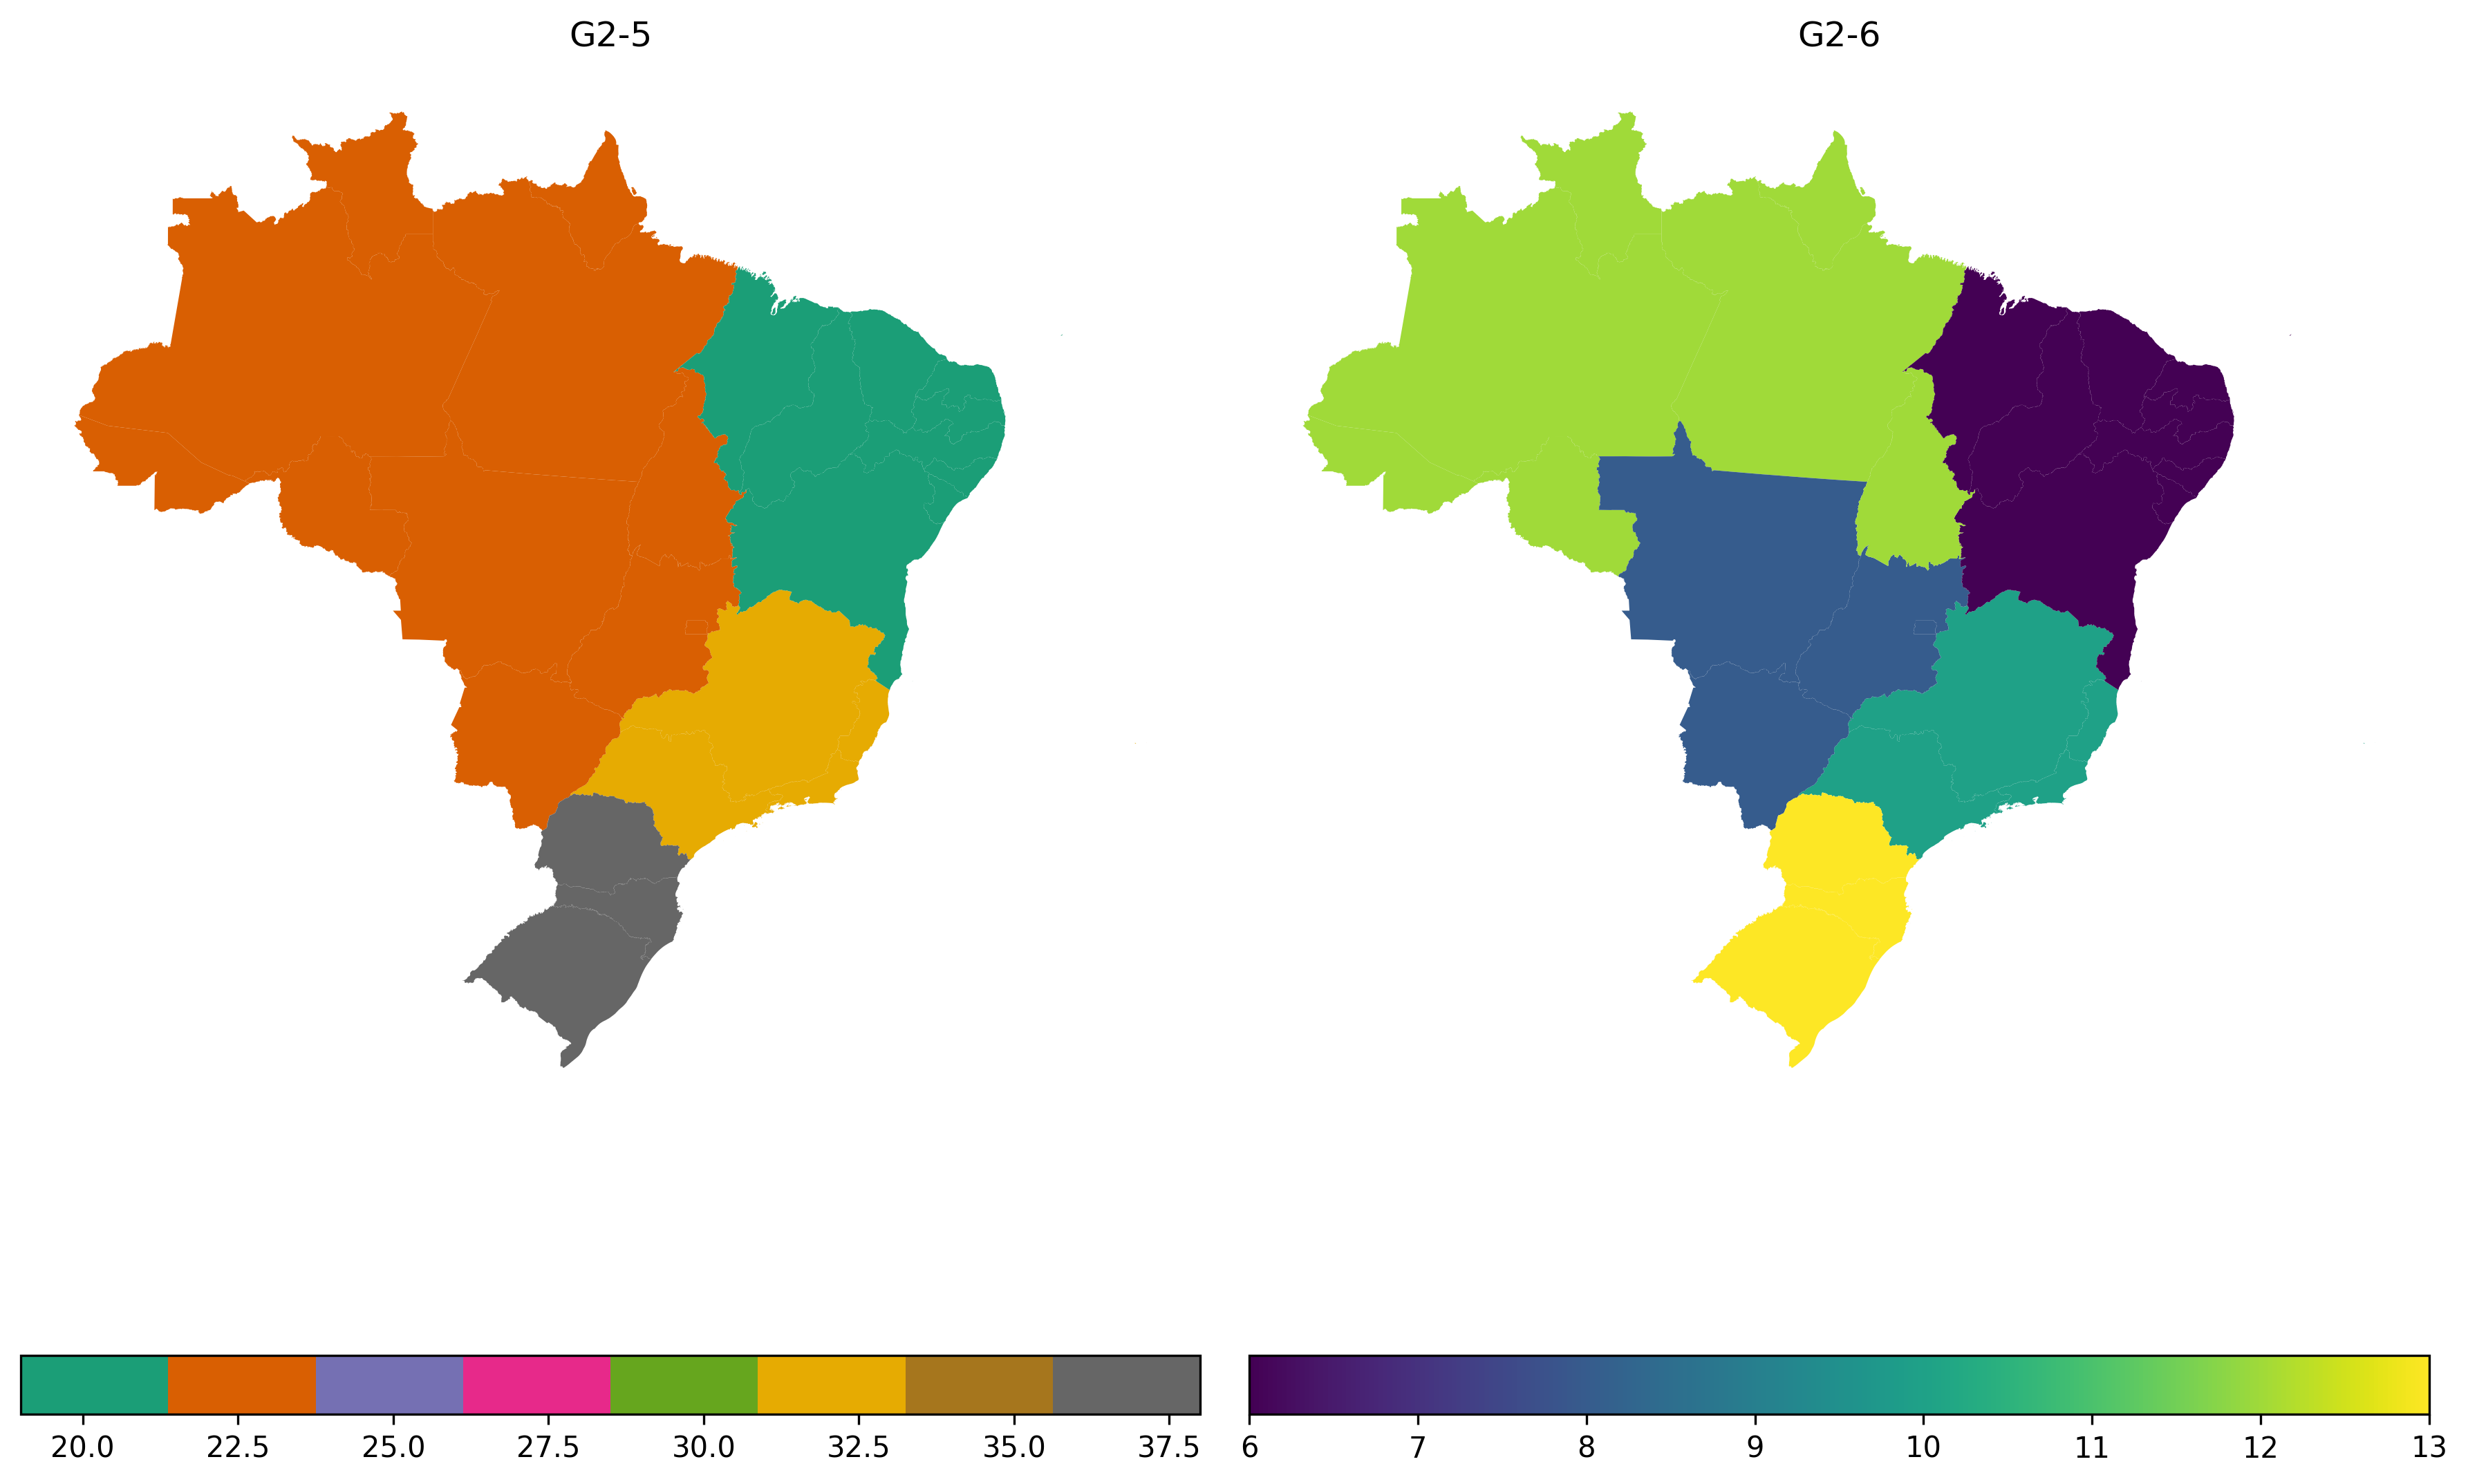
\includegraphics[width=1\linewidth]{figuras/mapa_coropletico_tic_domicilios_2024_g2_5_6.png}
	\label{fig:mapa_coropletico_tic_domicilios_2024_g2_5_6}
	\footnotesize{Fonte: \cite{tic_domicilios_2024_g2}.}
\end{figure}

Quando se trata do indicador G2-5, apenas as regiões Sudeste e Sul foram as que mais usaram serviços públicos relativos a impostos e taxas governamentais, como declaração de imposto de renda, IPVA ou IPTU.

Quando se trata do indicador G2-6, apenas a região Sul foi a que mais usou serviços públicos relativos à polícia e segurança, como boletim de ocorrência, antecedentes criminais ou denúncias.

\begin{figure}[H]
	\centering
	\caption{Indicador G2: critério 7}
	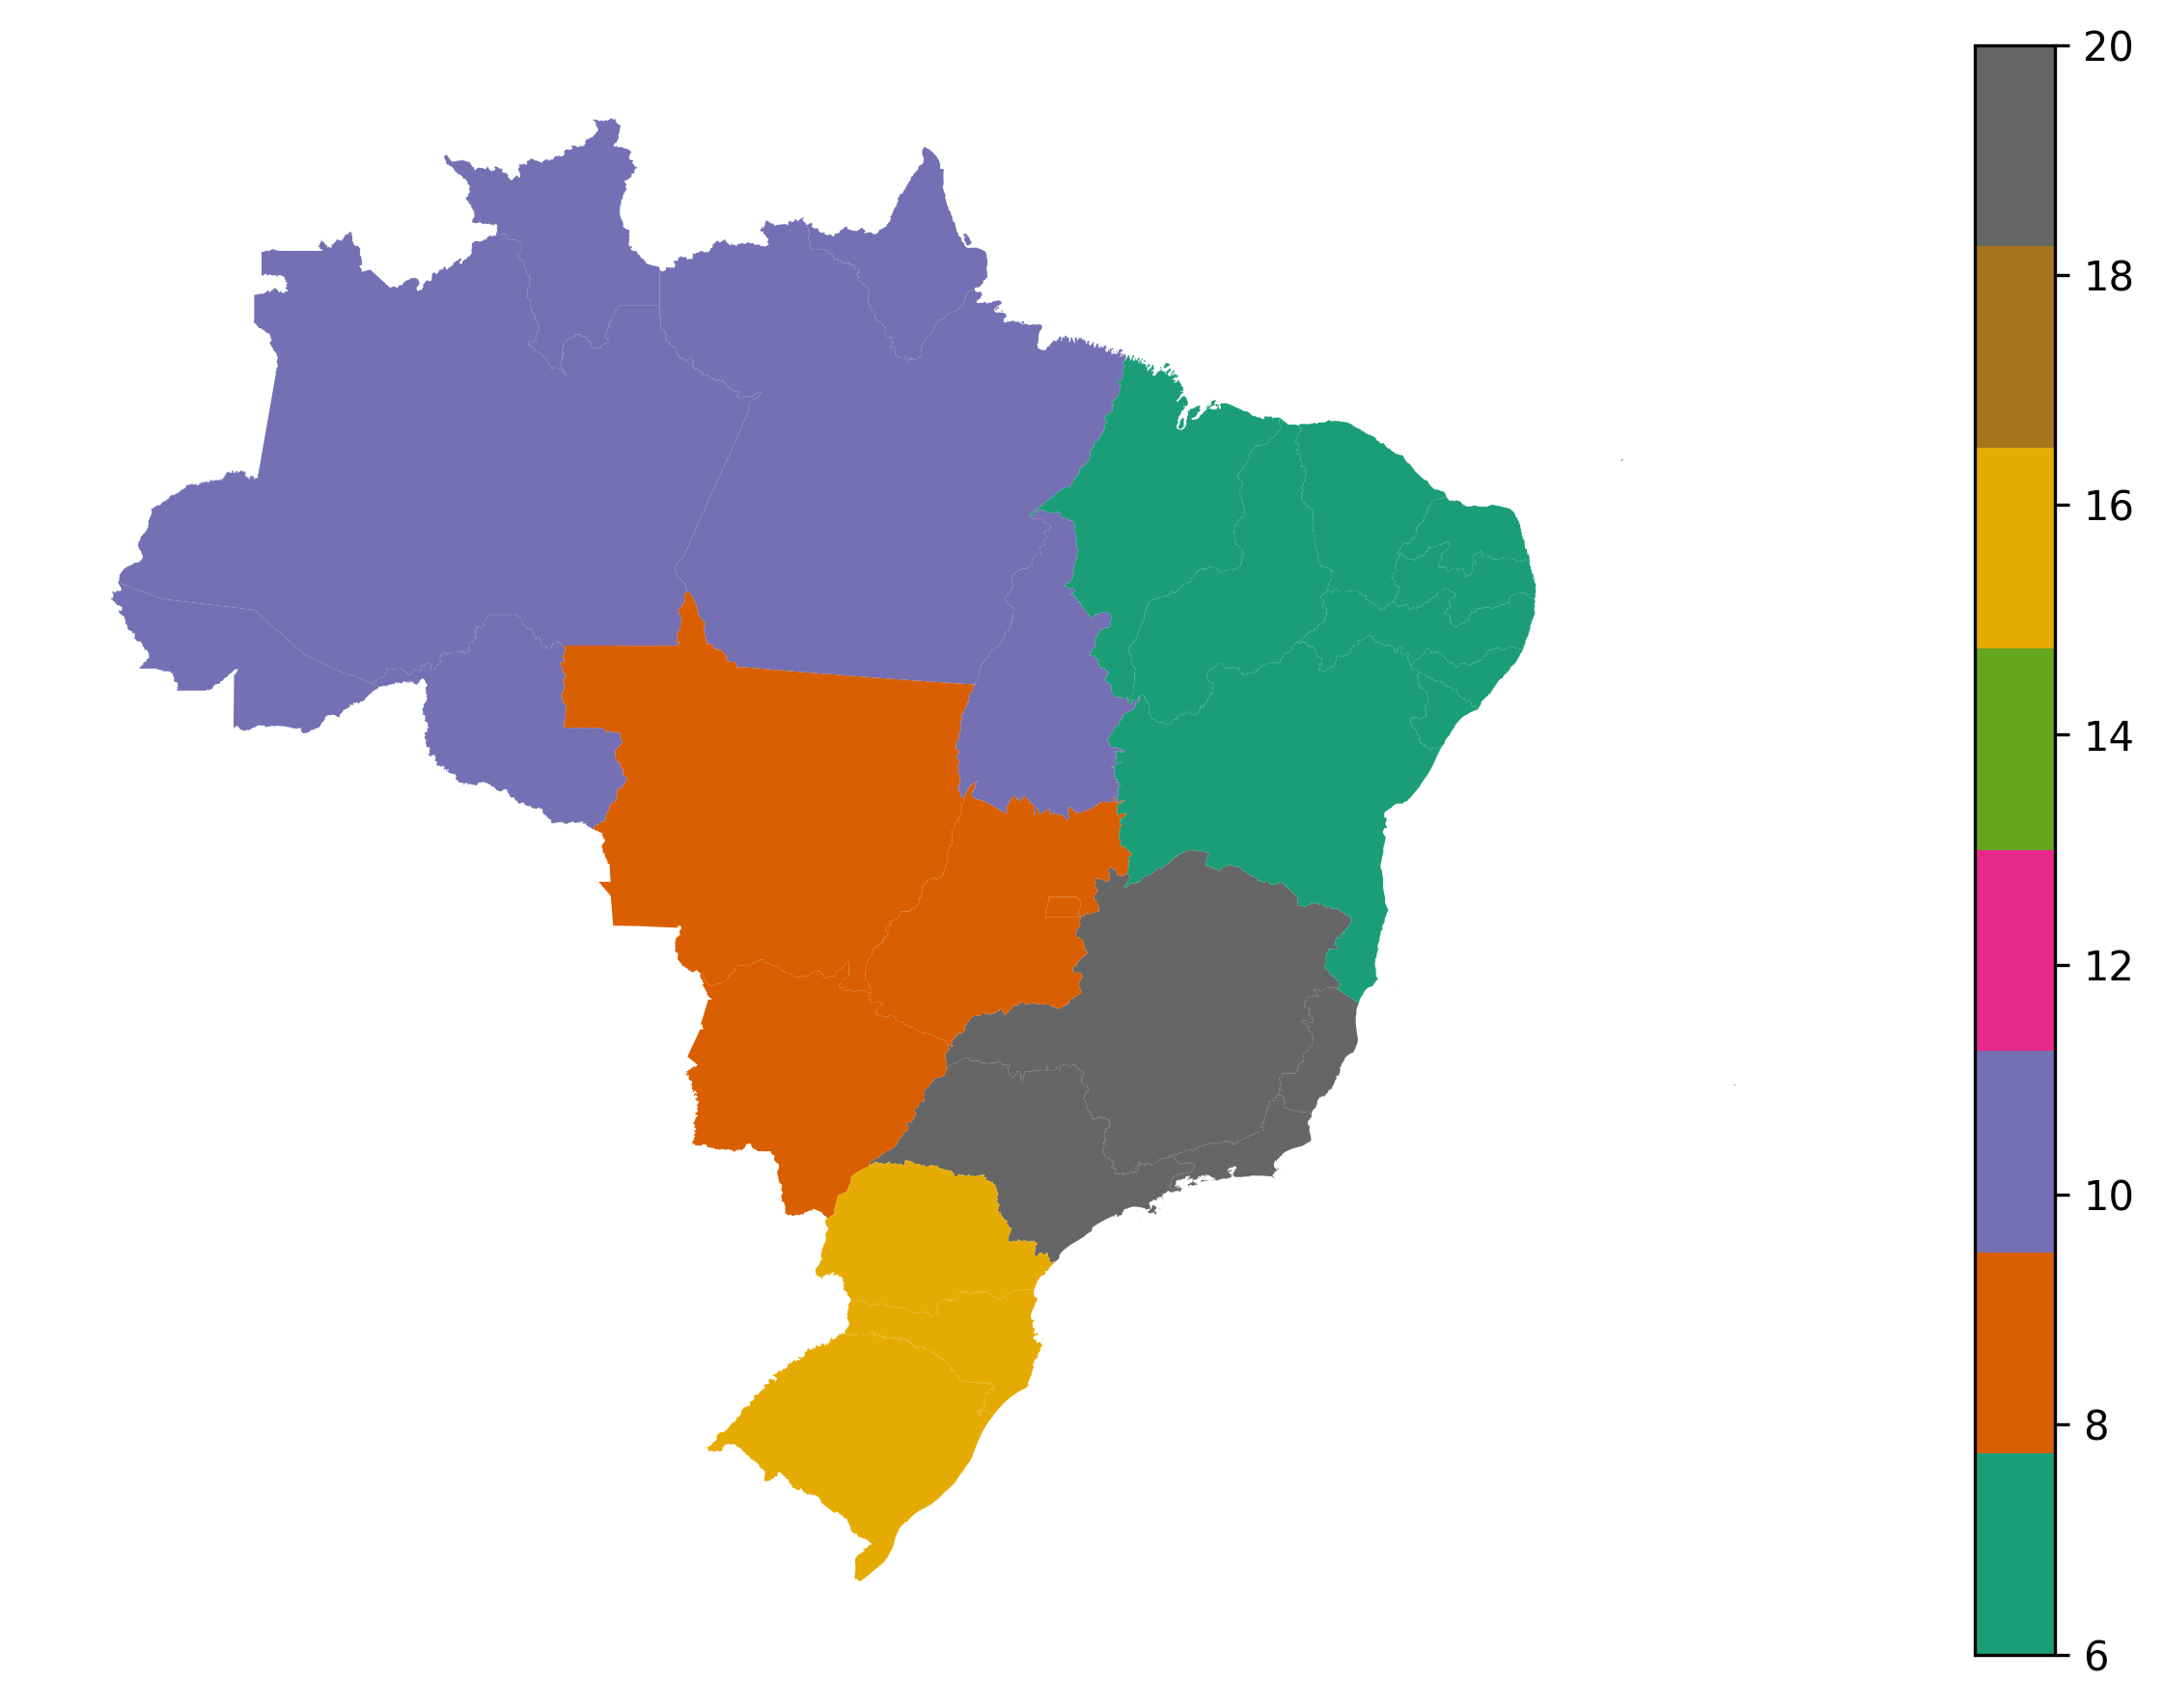
\includegraphics[width=1\linewidth]{figuras/mapa_coropletico_tic_domicilios_2024_g2_7.png}
	\label{fig:mapa_coropletico_tic_domicilios_2024_g2_7}
	\footnotesize{Fonte: \cite{tic_domicilios_2024_g2}.}
\end{figure}

Quando se trata do indicador G2-7, as regiões Sudeste e Sul foram as únicas que mais usaram serviços públicos relativos a transporte público ou outros serviços urbanos, como limpeza e conservação de vias e iluminação.

Complementar ao indicador G2, o indicador G2A detalha se o serviço público foi realizado, completamente ou parcialmente, na internet, e se apenas informações do serviço público foram procuradas na internet, incluídas as opções em que o questionado não respondeu ou não sabe, todos como subcritérios. 

O indicador G2A tem 7 critérios, conforme exposto pela figura \ref{fig:tabela_tic_domicilios_2024_criterios_g2a}.

\begin{figure}[H]
	\centering
	\caption{Critérios do indicador G2A}
	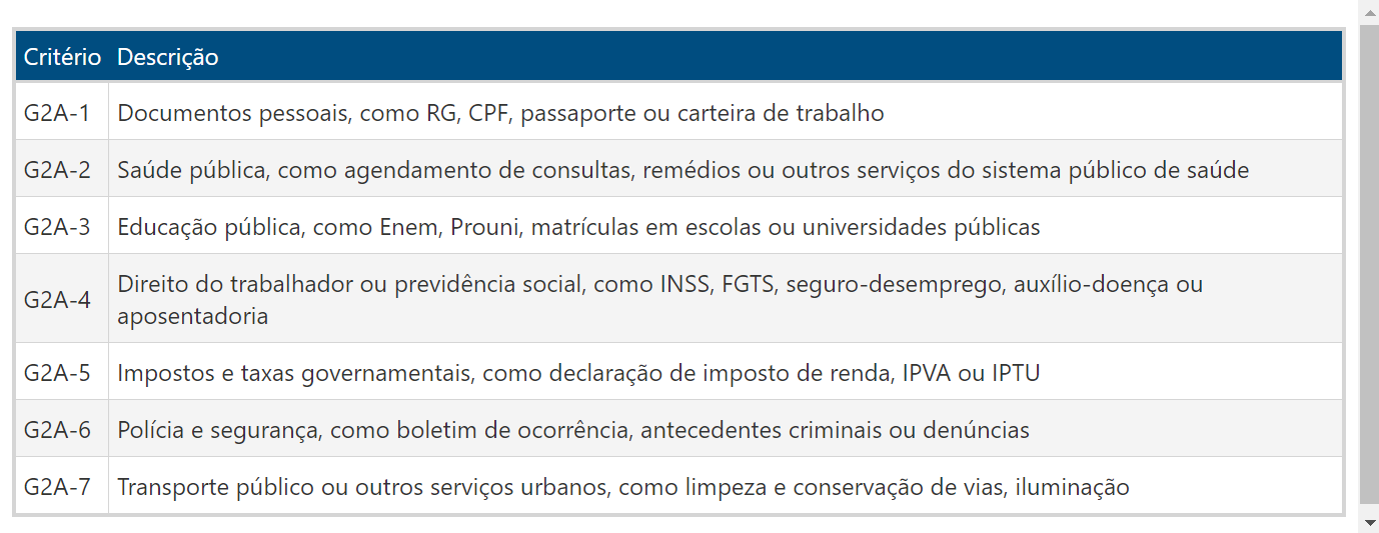
\includegraphics[width=1\linewidth]{figuras/tabela_tic_domicilios_2024_criterios_g2a.png}
	\label{fig:tabela_tic_domicilios_2024_criterios_g2a}
	\footnotesize{Fonte: \cite{tic_domicilios_2024_g2a}.}
\end{figure}

Os subcritérios do indicador G2A são, segundo \cite{tic_domicilios_2024_g2a}:

\begin{itemize}
    \item Realizou serviço na Internet sem precisar ir até um posto (SC1);  \item Realizou parte do serviço na Internet, mas precisou ir a um posto para finalizar (SC2);
    \item Apenas procurou informações na Internet (SC3);
    \item Não sabe; e
    \item Não respondeu.
\end{itemize}

As figuras \ref{fig:mapa_coropletico_tic_domicilios_2024_g2a_1}, \ref{fig:mapa_coropletico_tic_domicilios_2024_g2a_2}, \ref{fig:mapa_coropletico_tic_domicilios_2024_g2a_3},
\ref{fig:mapa_coropletico_tic_domicilios_2024_g2a_4},
\ref{fig:mapa_coropletico_tic_domicilios_2024_g2a_5} contêm mapa coropléticos que demonstram os subcritérios dos indicadores do G2A, que não incluirão as opções \textbf{não respondeu} e \textbf{não sabe}.

\begin{figure}[H]
	\centering
	\caption{Indicador G2A: critério 1}
	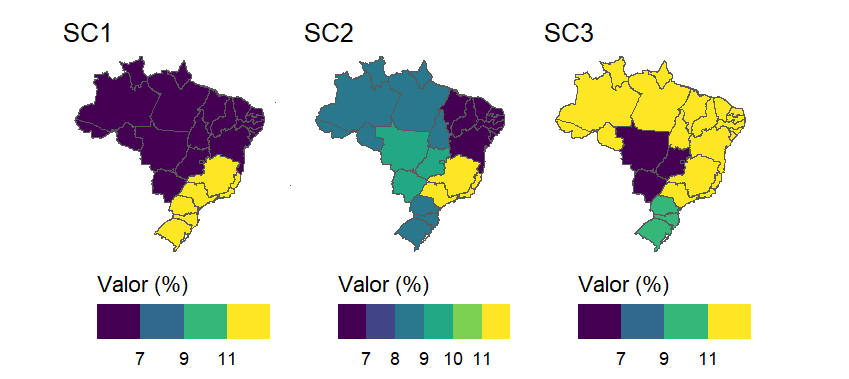
\includegraphics[width=1\linewidth]{figuras/mapa_coropletico_tic_domicilios_2024_g2a_1.png}
	\label{fig:mapa_coropletico_tic_domicilios_2024_g2a_1}
	\footnotesize{Fonte: \cite{tic_domicilios_2024_g2a}.}
\end{figure}

No tocante ao SC1, as regiões Sudeste e Sul foram as regiões em que mais ocorreram serviços na internet sem precisar ir até um posto. 

No tocante ao SC2, a região Sudeste foi a única região em que mais foram realizados partes dos serviços na Internet, mas foi preciso ir a um posto para finalizar, seguida do Centro-Oeste e das regiões Norte e Sul.

No tocante ao SC3, as regiões Norte, Nordeste, Sudeste foram as regiões em que mais se procurou informações na internet, seguidas do Sul e do Centro-Oeste.

\begin{figure}[H]
	\centering
	\caption{Indicador G2A: critério 2}
	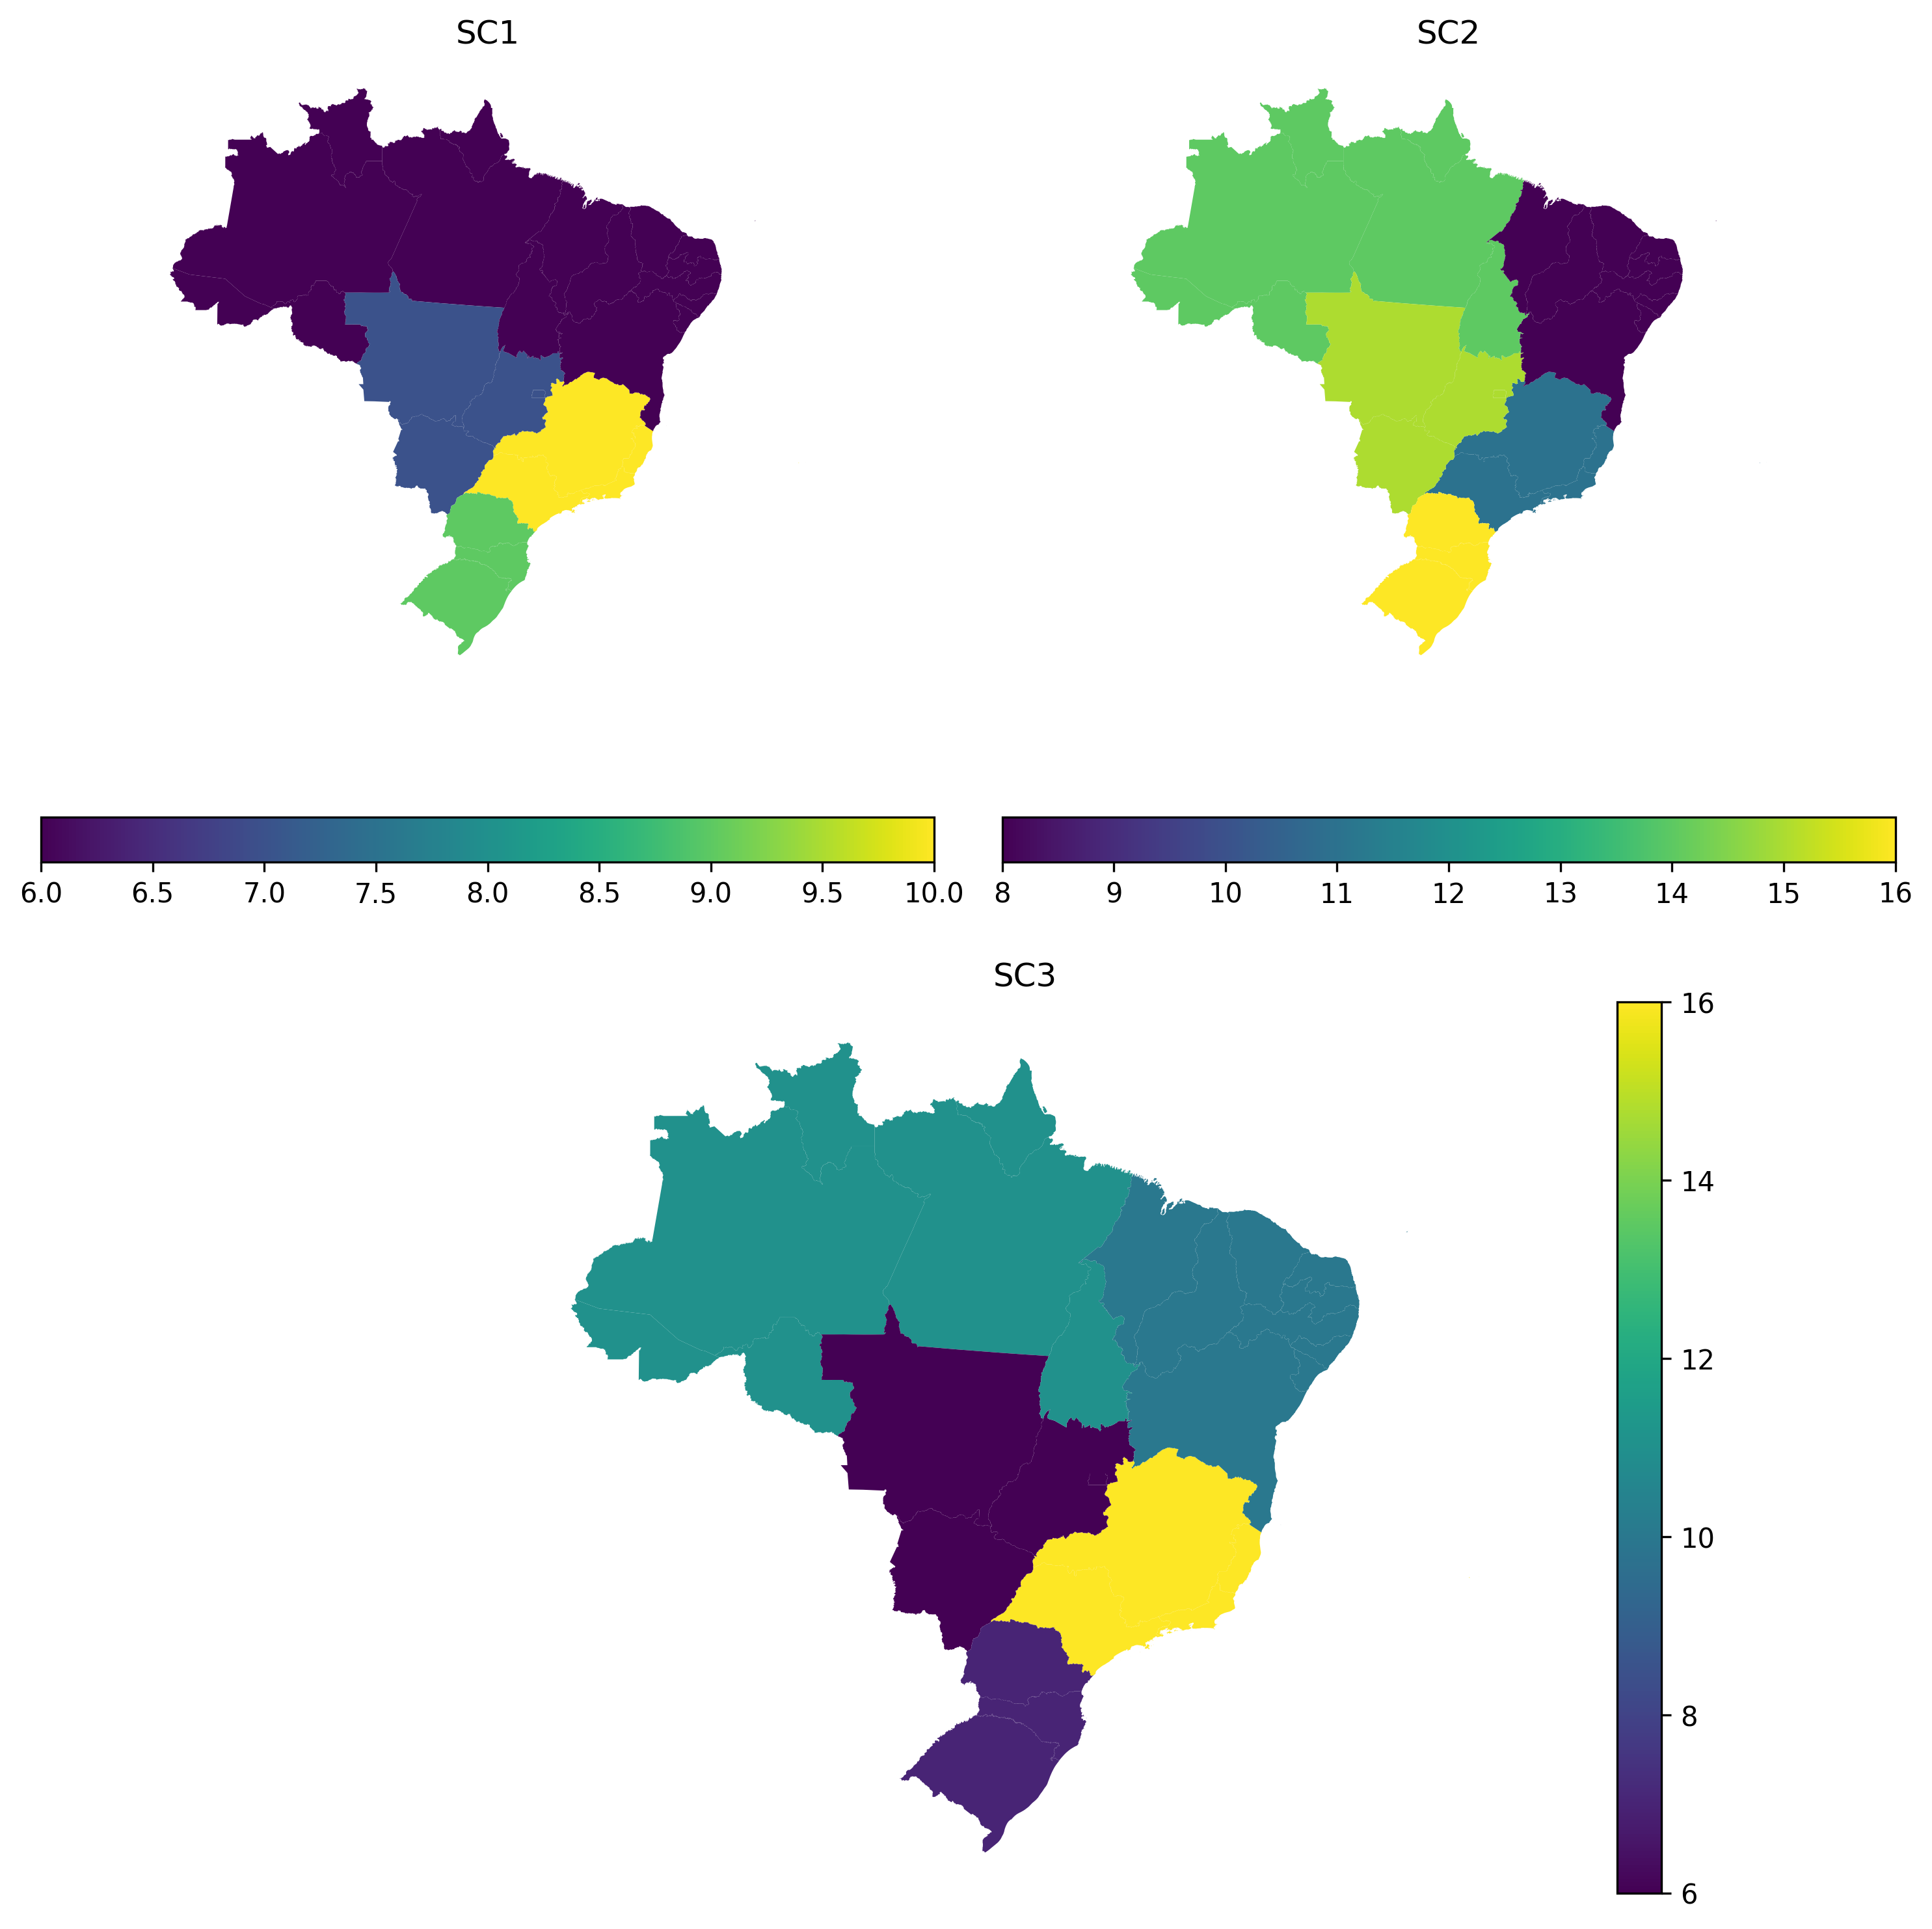
\includegraphics[width=1\linewidth]{figuras/mapa_coropletico_tic_domicilios_2024_g2a_2.png}
	\label{fig:mapa_coropletico_tic_domicilios_2024_g2a_2}
	\footnotesize{Fonte: \cite{tic_domicilios_2024_g2a}.}
\end{figure}

No tocante ao SC1, as regiões Sudeste e Sul foram as regiões em que mais ocorreram serviços na internet sem precisar ir até um posto.

No tocante ao SC2, a região Sudeste foi a região em que mais foram realizados partes dos serviços na Internet, mas foi preciso ir a um posto para finalizar, seguidas  das regiões Sul e Norte, e por fim, do Centro-Oeste.

No tocante ao SC3, a região Sudeste foi a região em que mais se procurou informações na internet, seguida do Nordeste e Norte, bem como, conjuntamente, o Centro-Oeste e o Sul.

\begin{figure}[H]
	\centering
	\caption{Indicador G2A: critério 3}
	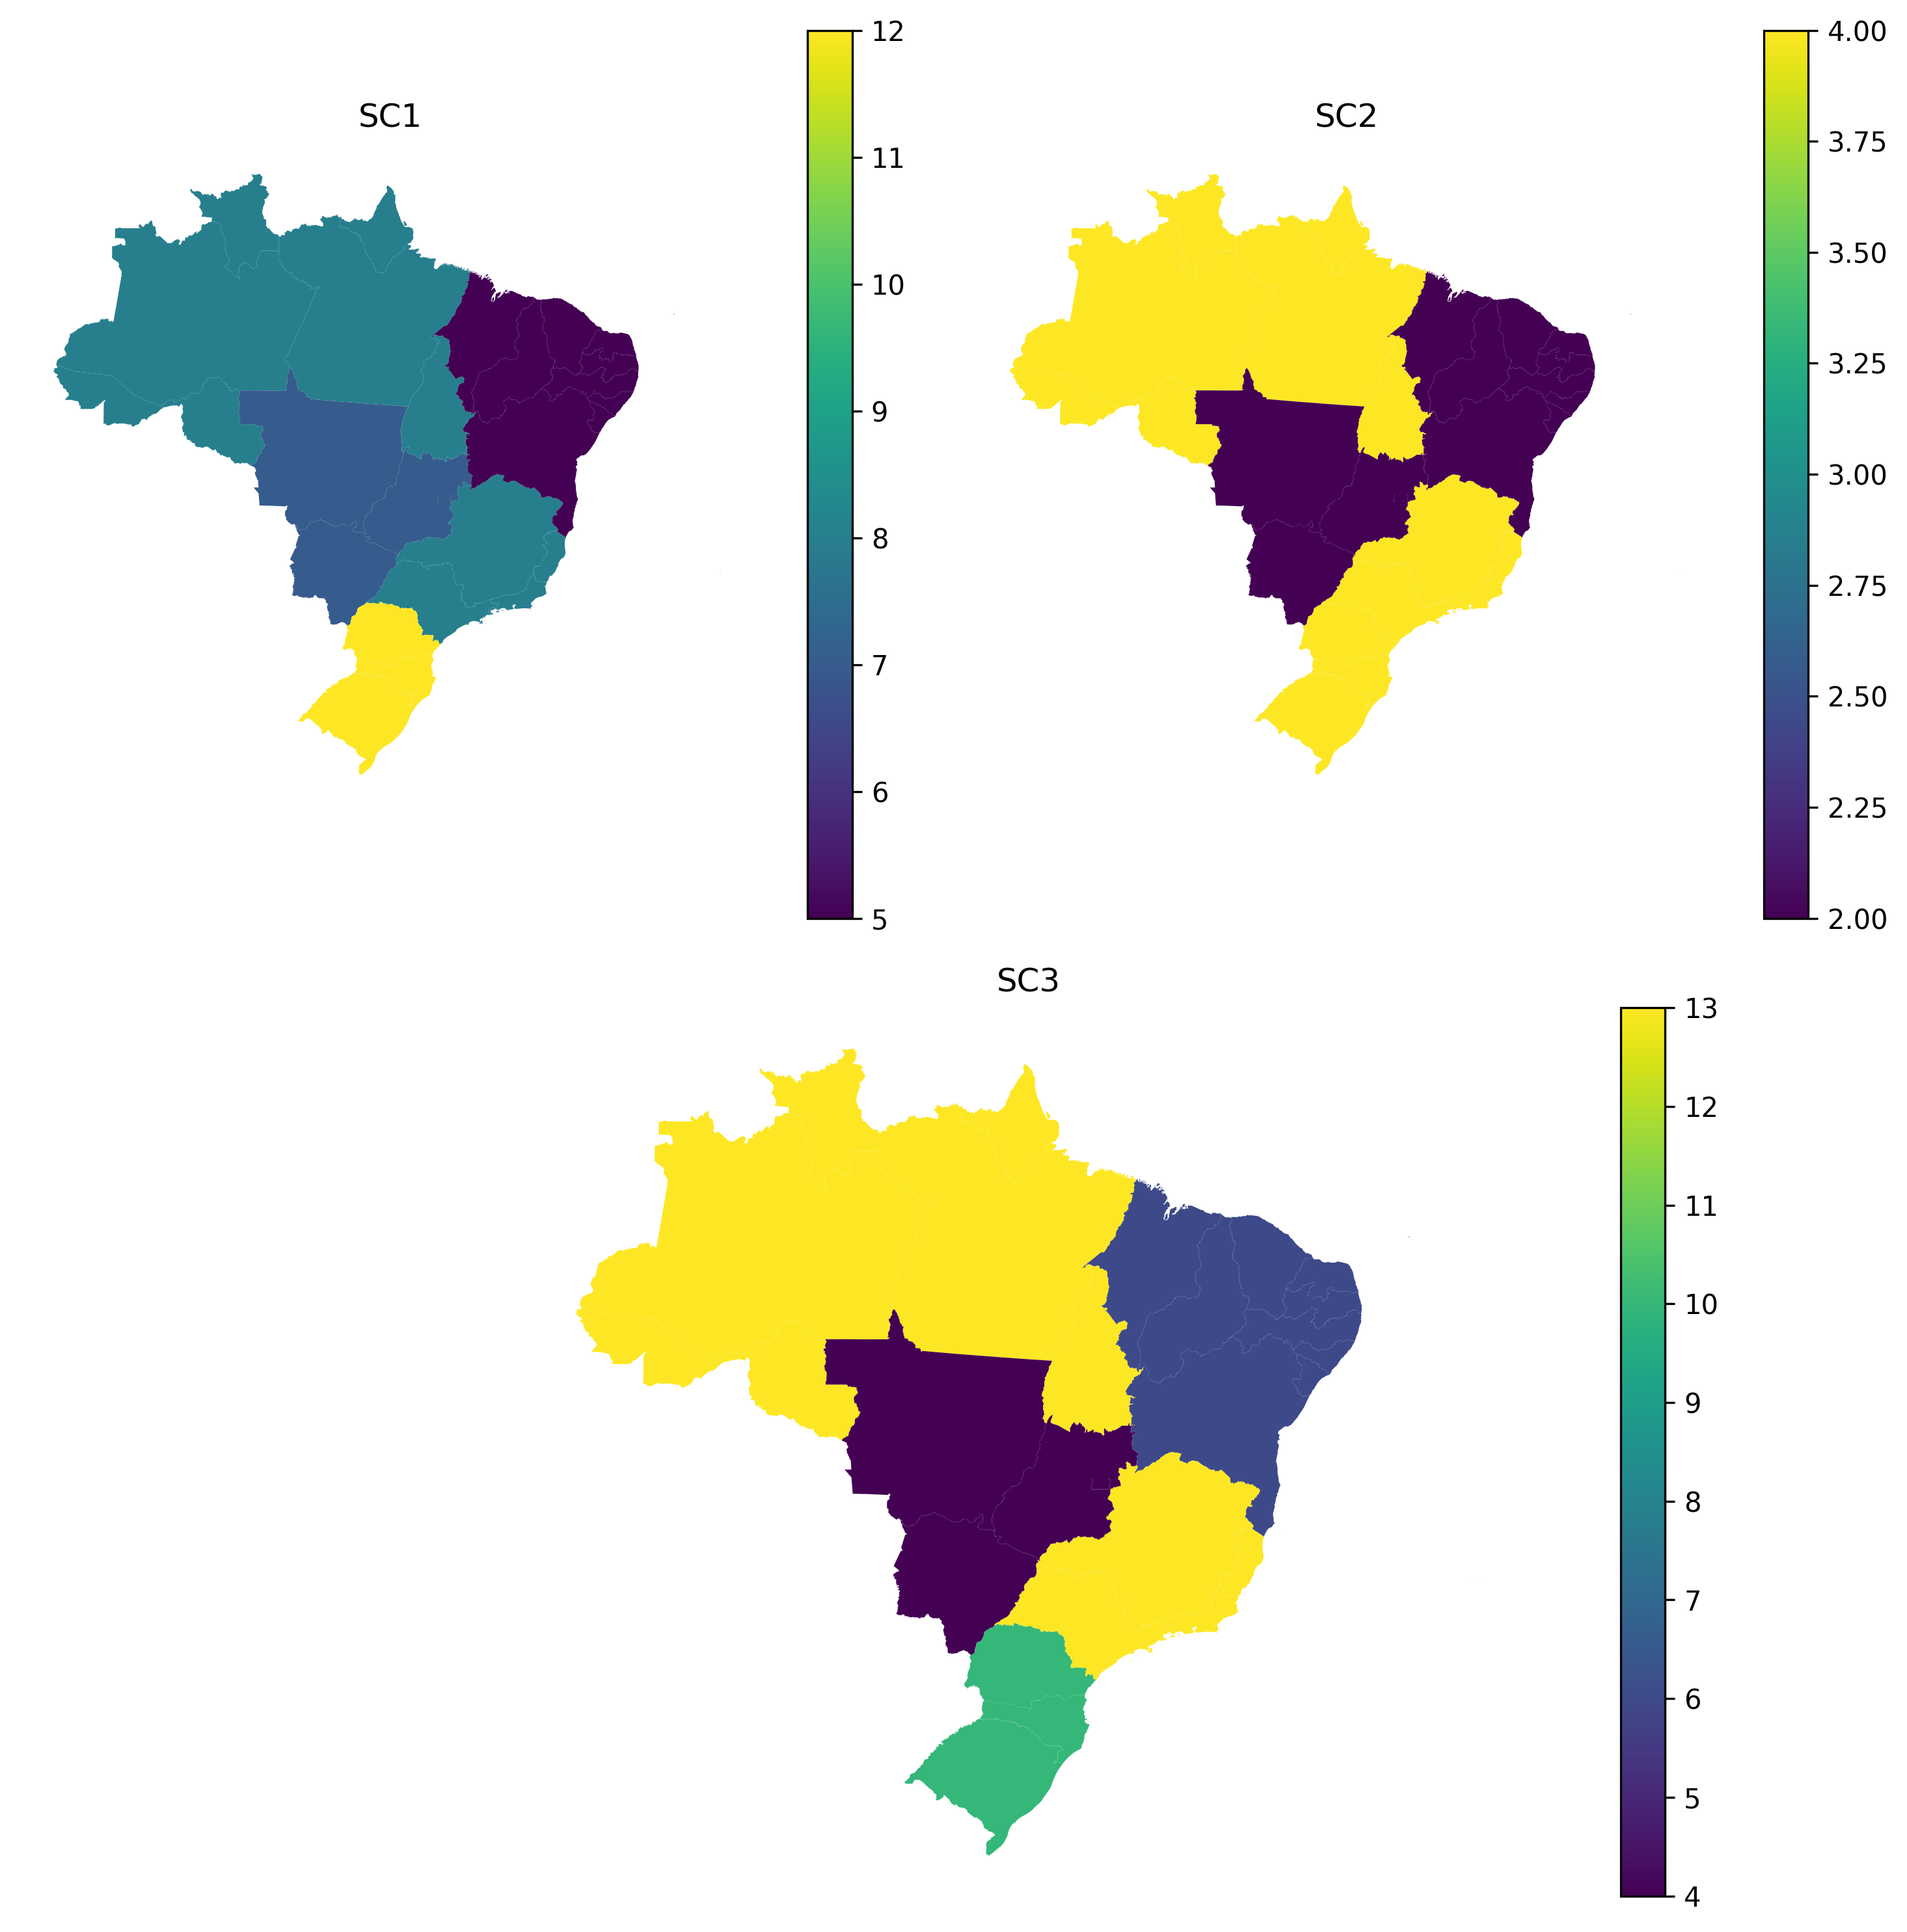
\includegraphics[width=1\linewidth]{figuras/mapa_coropletico_tic_domicilios_2024_g2a_3.png}
	\label{fig:mapa_coropletico_tic_domicilios_2024_g2a_3}
	\footnotesize{Fonte: \cite{tic_domicilios_2024_g2a}.}
\end{figure}

No tocante ao SC1, a região Sul foi a região em que mais ocorreram serviços na internet sem precisar ir até um posto, sendo o Nordeste a região em que mais se foi presencialmente aos postos.

No tocante ao SC2, as regiões Norte, Sudeste e Sul foram as regiões em que mais foram realizados partes dos serviços na Internet, mas foi preciso ir a um posto para finalizar, seguidas do Nordeste e Centro-Oeste.

No tocante ao SC3, as regiões Norte e Sudeste em que mais se procurou informações na internet, seguidas do Nordeste e das regiões Centro-Oeste e Sul.

\begin{figure}[H]
	\centering
	\caption{Indicador G2A: critério 4}
	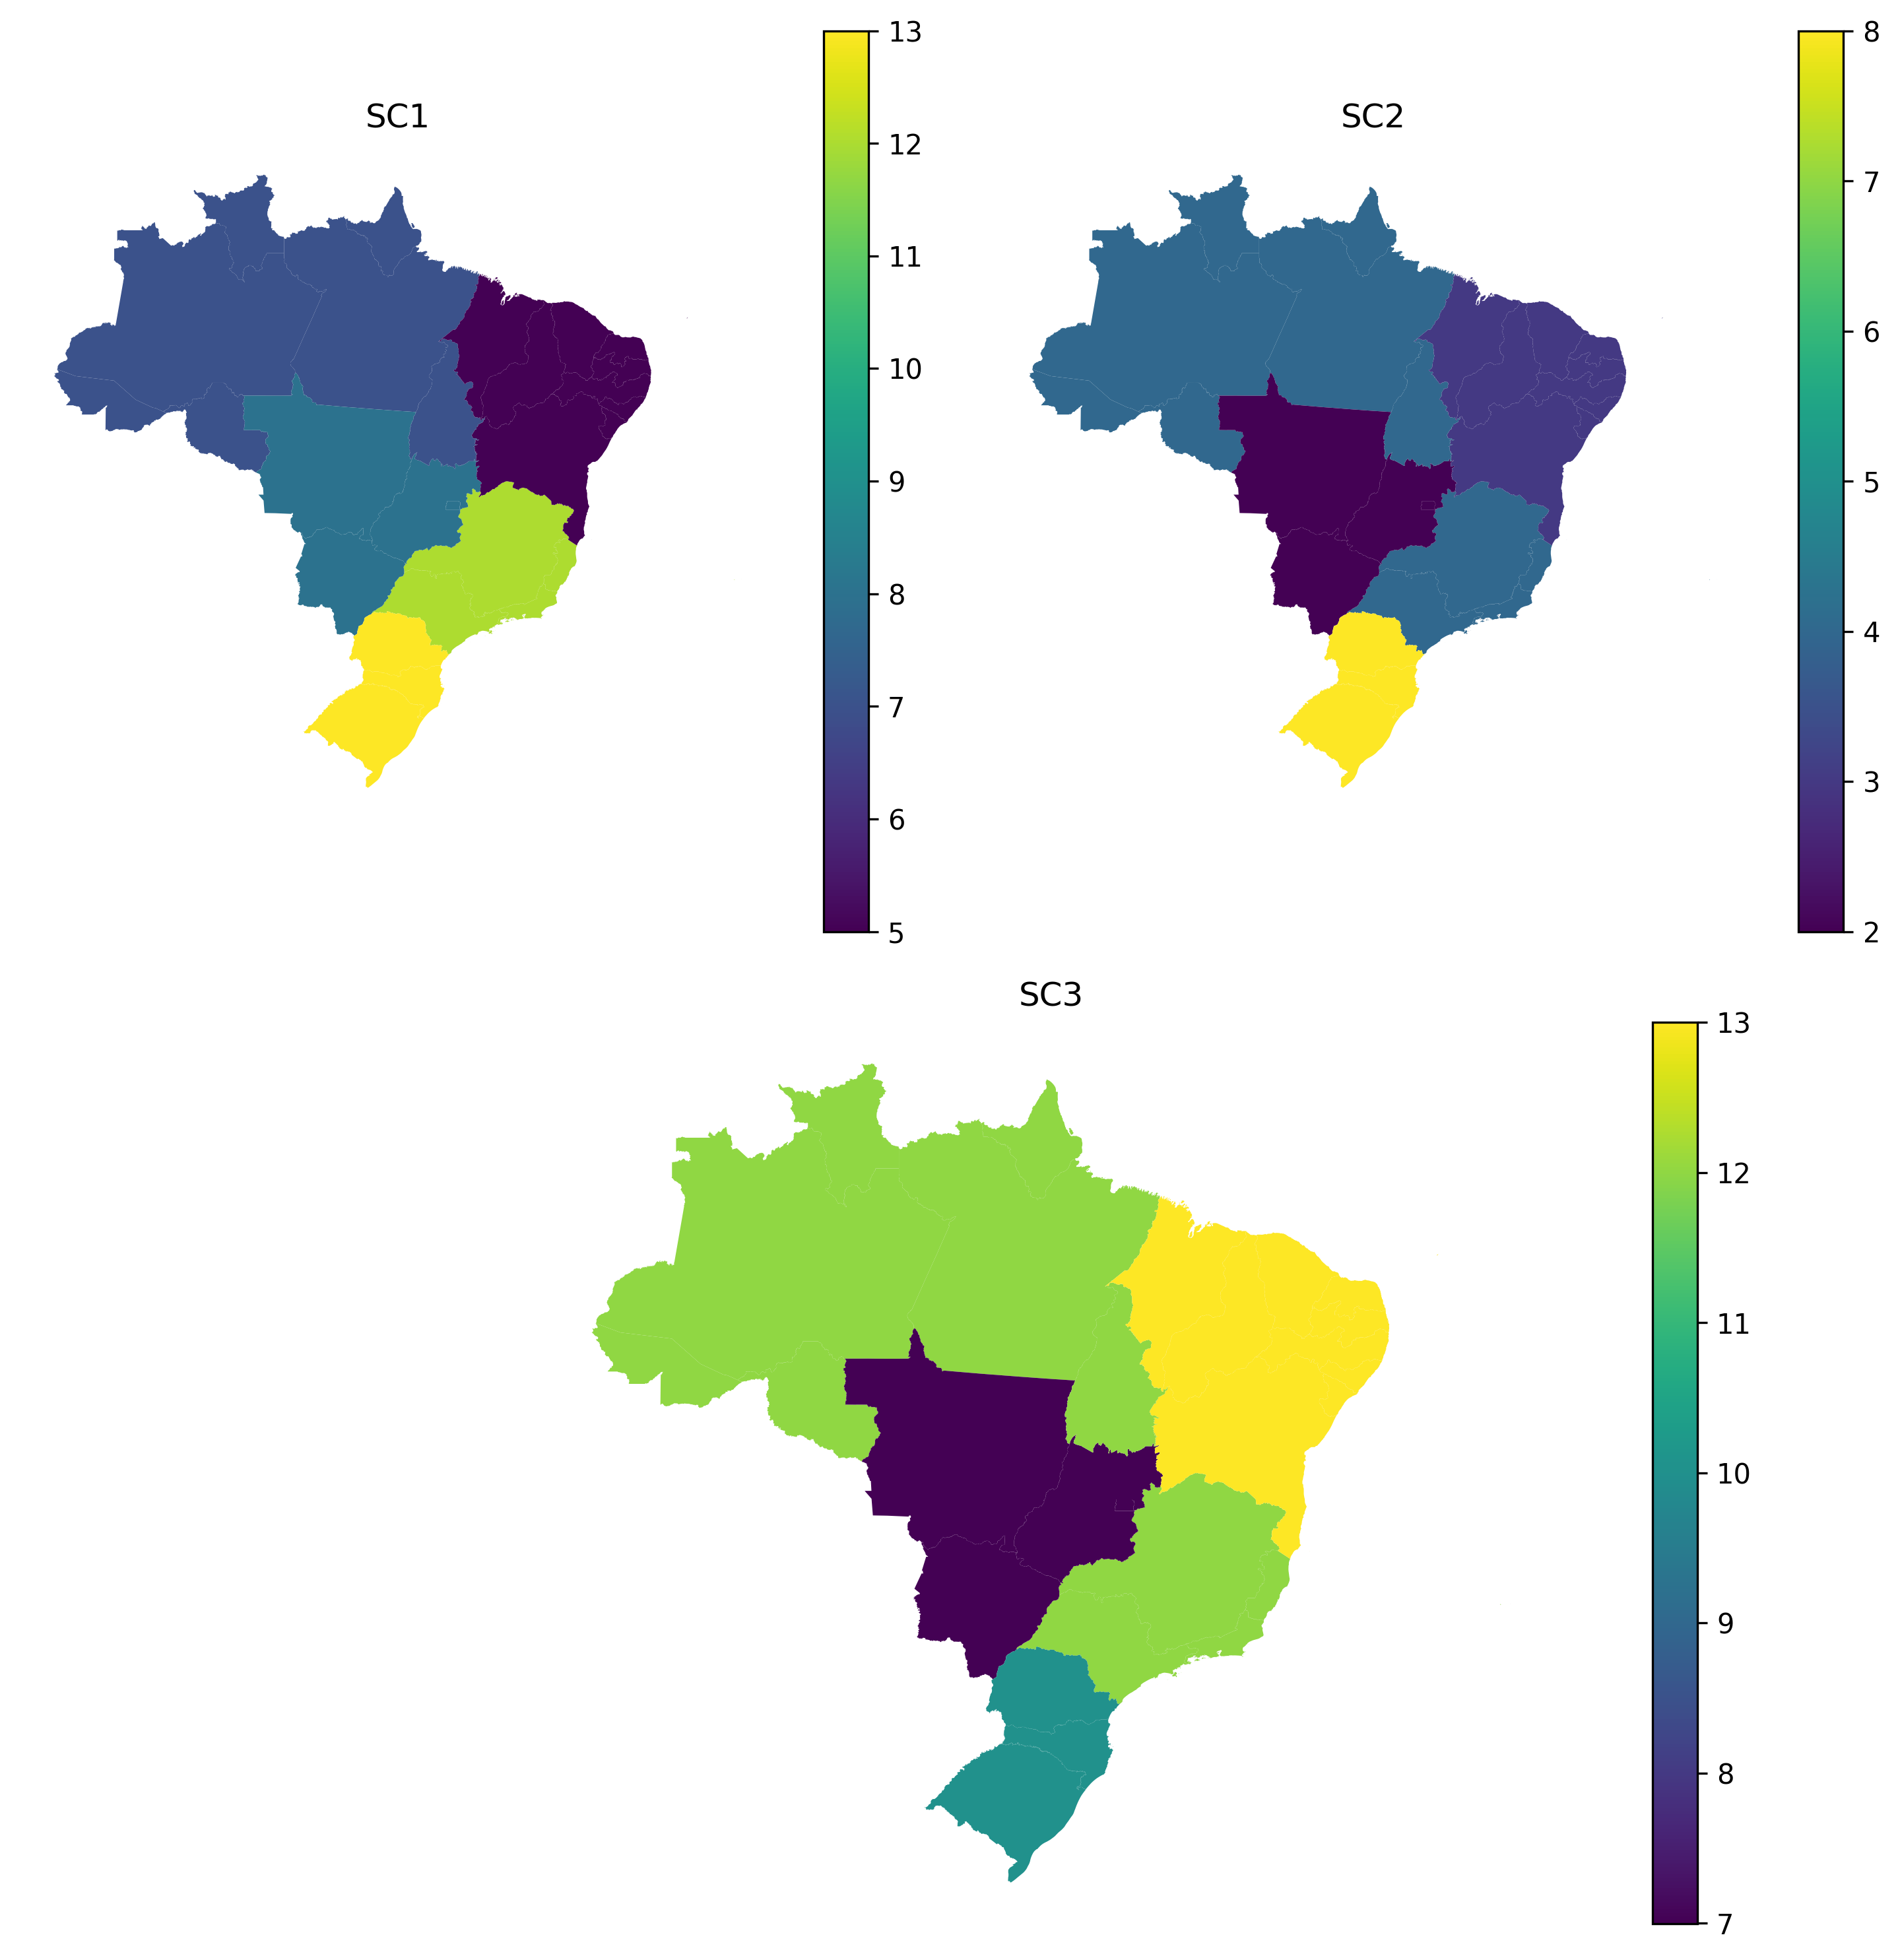
\includegraphics[width=1\linewidth]{figuras/mapa_coropletico_tic_domicilios_2024_g2a_4.png}
	\label{fig:mapa_coropletico_tic_domicilios_2024_g2a_4}
	\footnotesize{Fonte: \cite{tic_domicilios_2024_g2a}.}
\end{figure}

No tocante ao SC1, as regiões Sudeste e Sul foram as regiões em que mais ocorreram serviços na internet sem precisar ir até um posto, seguidas do Centro-Oeste e das regiões Norte e Nordeste.

No tocante ao SC2, a região Sul foi a região em que mais foram realizados partes dos serviços na Internet, mas foi preciso ir a um posto para finalizar, seguidas do Sudeste e Norte e das regiões Centro-Oeste e Nordeste.

No tocante ao SC3, a região Nordeste foi a região em que mais se procurou informações na internet, seguidas do Norte e Sudeste e da região Centro-Oeste.

\begin{figure}[H]
	\centering
	\caption{Indicador G2A: critério 5}
	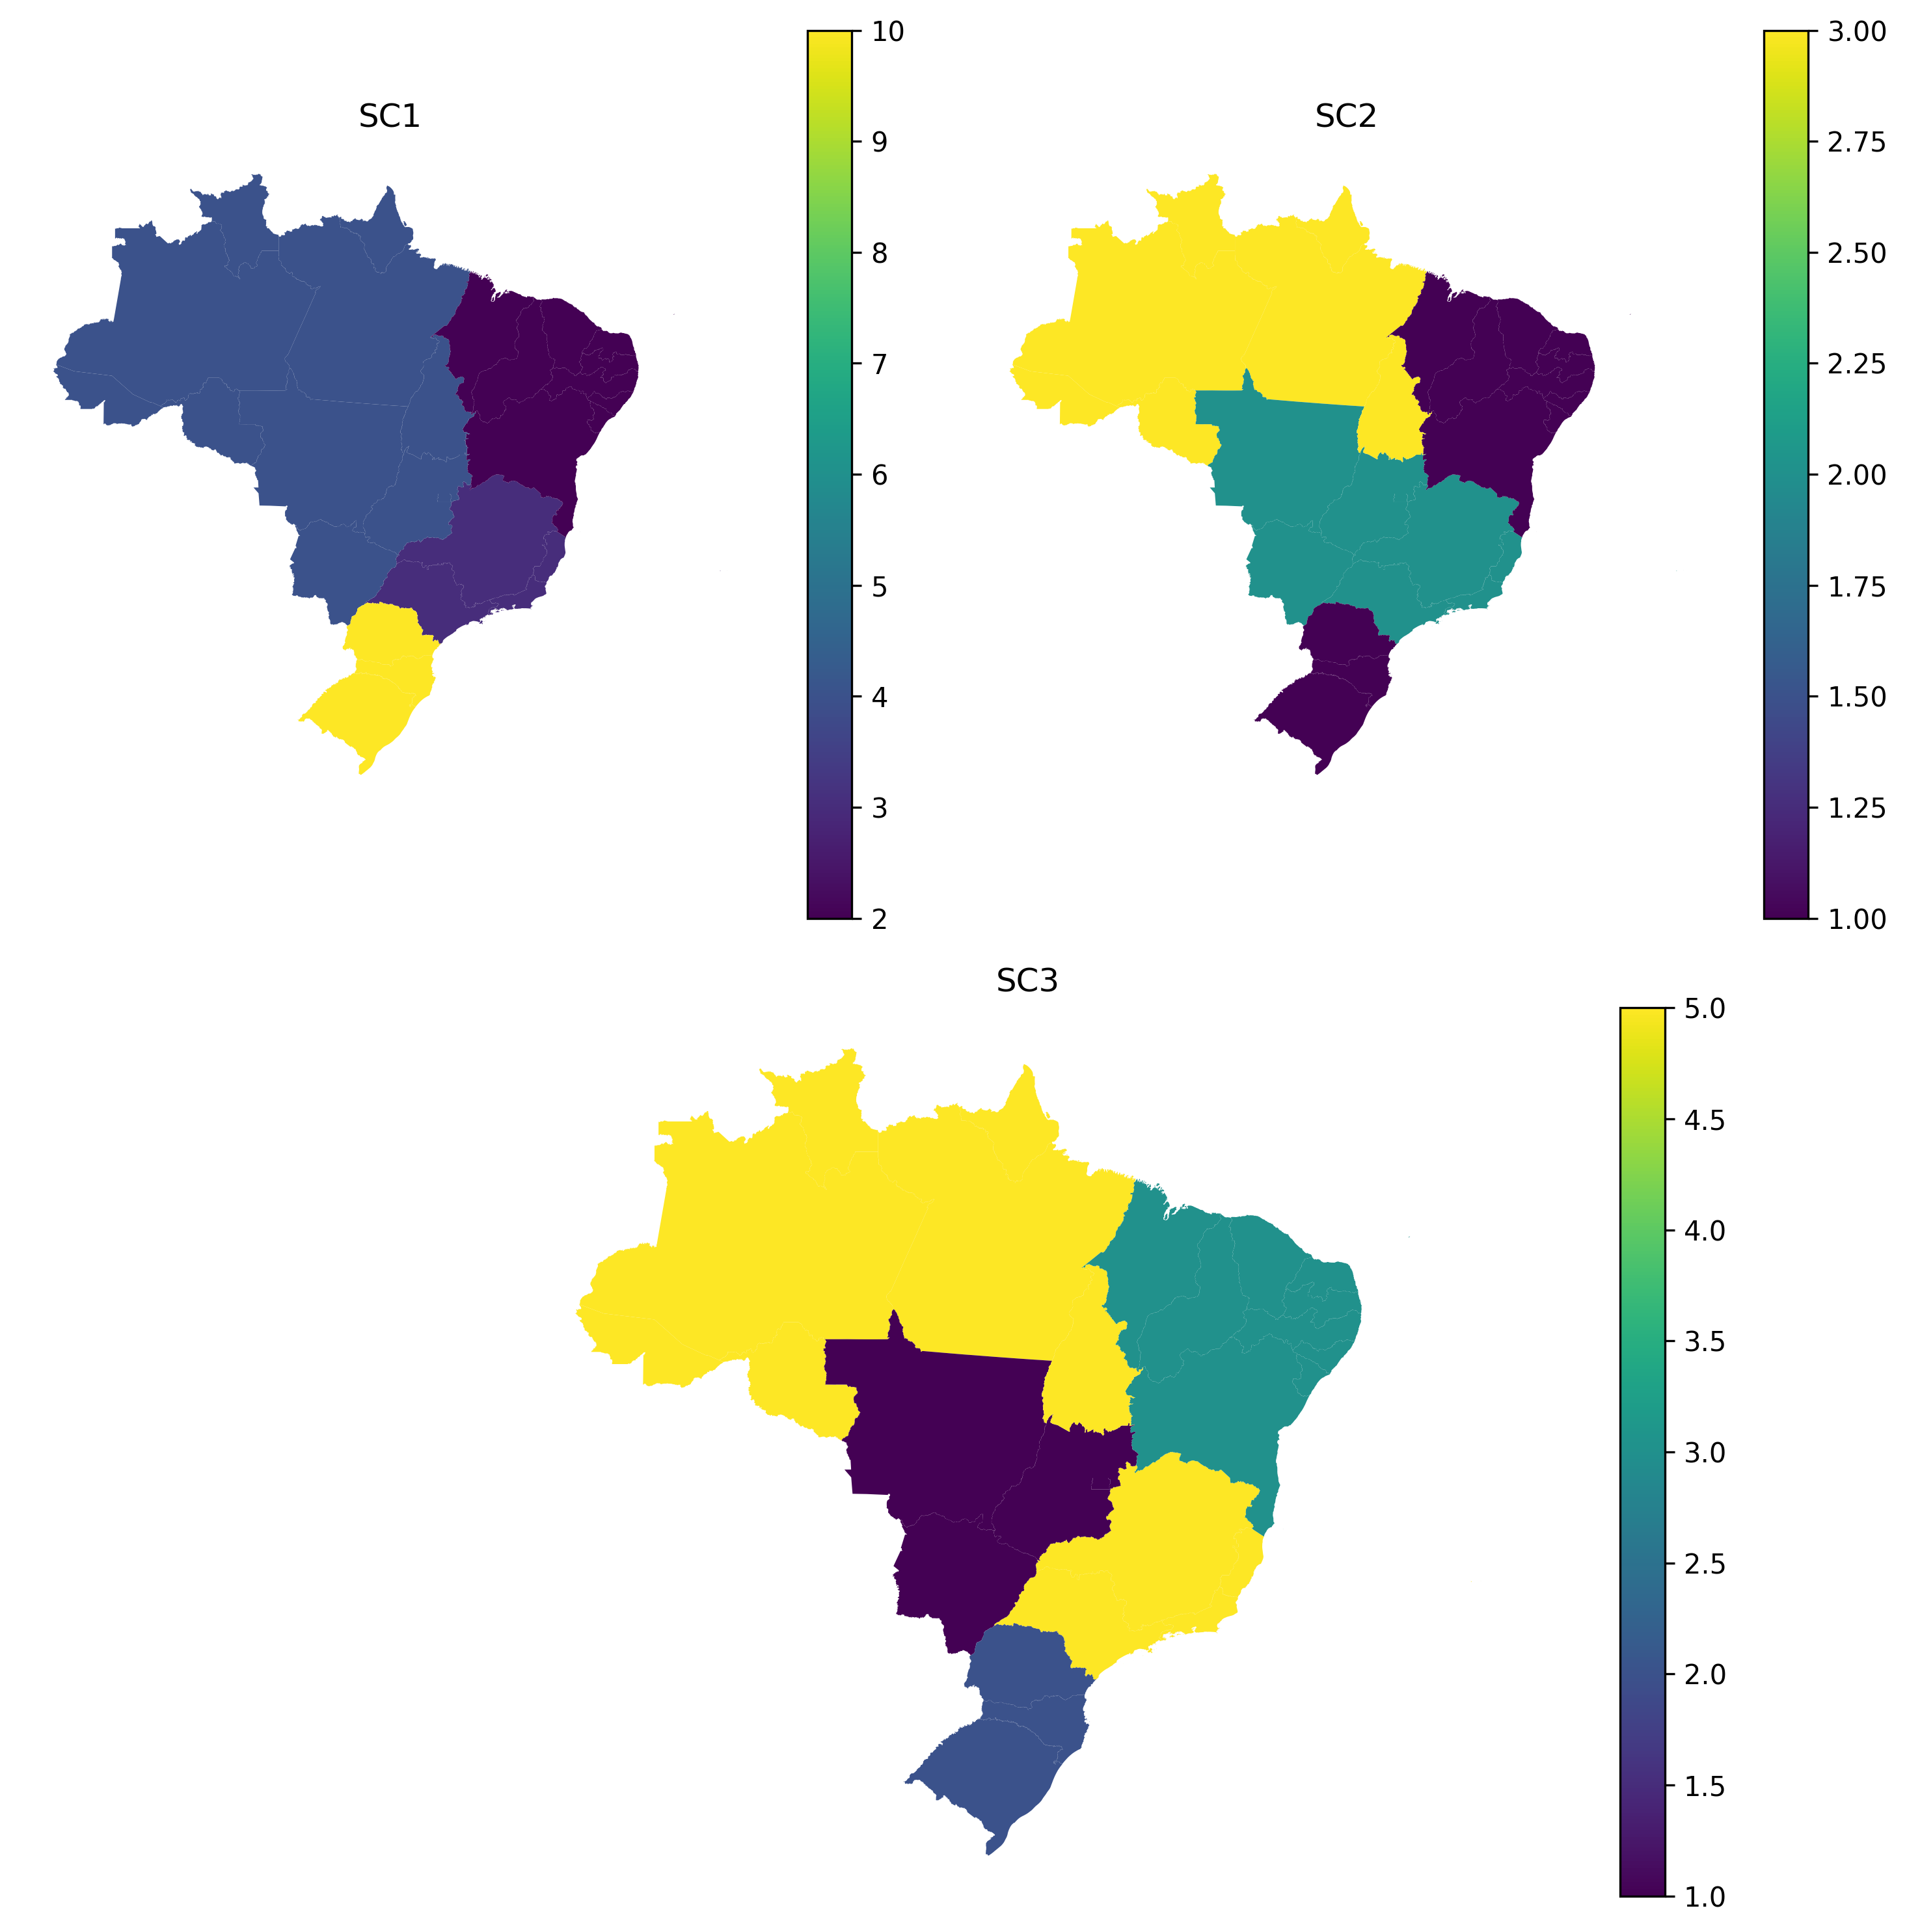
\includegraphics[width=1\linewidth]{figuras/mapa_coropletico_tic_domicilios_2024_g2a_5.png}
	\label{fig:mapa_coropletico_tic_domicilios_2024_g2a_5}
	\footnotesize{Fonte: \cite{tic_domicilios_2024_g2a}.}
\end{figure}

No tocante ao SC1, a região Sul foi a região em que mais ocorreram serviços na internet sem precisar ir até um posto, seguidas do Sudeste, Centro-Oeste e das regiões Norte e Nordeste.

No tocante ao SC2, a região Sul foi a região em que mais foram realizados partes dos serviços na Internet, mas foi preciso ir a um posto para finalizar, seguidas do Centro-Oeste e Norte e das regiões Sudeste e Nordeste.

No tocante ao SC3, as regiões Norte e Nordeste foram a região em que mais se procurou informações na internet, seguidas do Sudeste, Sul e da região Centro-Oeste.

\begin{figure}[H]
	\centering
	\caption{Indicador G2A: critério 6}
	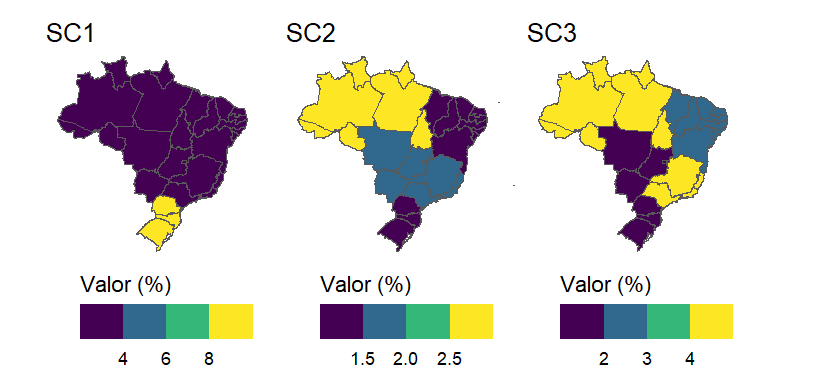
\includegraphics[width=1\linewidth]{figuras/mapa_coropletico_tic_domicilios_2024_g2a_6.png}
	\label{fig:mapa_coropletico_tic_domicilios_2024_g2a_6}
	\footnotesize{Fonte: \cite{tic_domicilios_2024_g2a}.}
\end{figure}

No tocante ao SC1, apenas a região Sul foi a região em que mais ocorreram serviços na internet sem precisar ir até um posto.

No tocante ao SC2, a região Norte foi a região em que mais foram realizados partes dos serviços na Internet, mas foi preciso ir a um posto para finalizar, seguidas do Centro-Oeste e Sudeste e das regiões Sul e Nordeste.

No tocante ao SC3, as regiões Norte e Sudeste foram a região em que mais se procurou informações na internet, seguidas do Nordeste e das regiões Centro-Oeste e Sul.

\begin{figure}[H]
	\centering
	\caption{Indicador G2A: critério 7}
	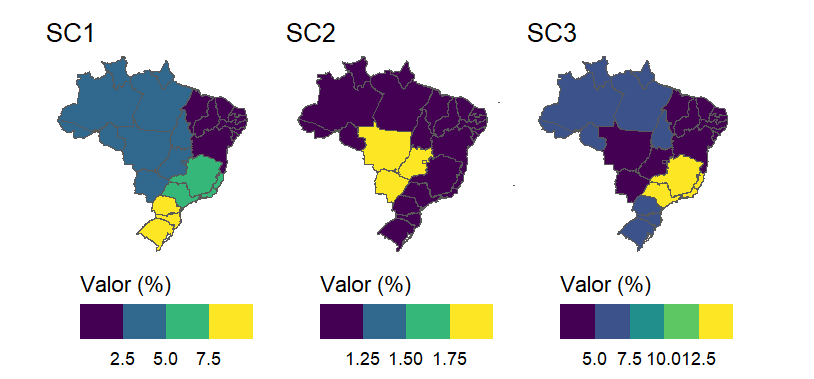
\includegraphics[width=1\linewidth]{figuras/mapa_coropletico_tic_domicilios_2024_g2a_7.png}
	\label{fig:mapa_coropletico_tic_domicilios_2024_g2a_7}
	\footnotesize{Fonte: \cite{tic_domicilios_2024_g2a}.}
\end{figure}

No tocante ao SC1, a região Sul foi a região em que mais ocorreram serviços na internet sem precisar ir até um posto, seguidas das regiões Sudeste, conjuntamente, o Centro-Oeste e o Norte, e por fim, o Nordeste.

No tocante ao SC2, apenas a região Centro-Oeste foi a região em que mais foram realizados partes dos serviços na Internet.

No tocante ao SC3, as regiões Norte e Sudeste foram a região em que mais se procurou informações na internet, seguidas do Nordeste e das regiões Centro-Oeste e Sul.

Terminando a análise do TIC Domicílios 2024, analisar-se-á o indicador G3. O indicador representa os usuários de internet, por atividades de interação com autoridades públicas.

figura \ref{fig:tabela_tic_domicilios_2024_criterios_g3} contém a tabela com a descrição dos seus 3 critérios.  

\begin{figure}[H]
	\centering
	\caption{Critérios do Indicador G3}
	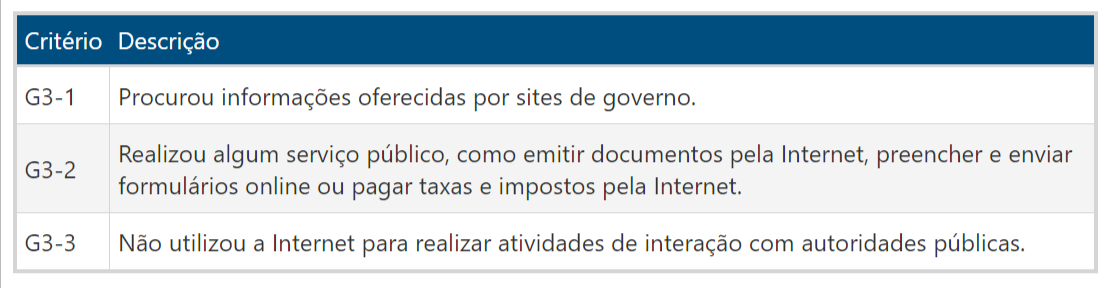
\includegraphics[width=1\linewidth]{figuras/tabela_tic_domicilios_2024_criterios_g3.png}
	\label{fig:tabela_tic_domicilios_2024_criterios_g3}
	\footnotesize{Fonte: elaboração própria baseade em \cite{tic_domicilios_2024_g3}.}
\end{figure}

Haja vista a figura \ref{fig:tabela_tic_domicilios_2024_criterios_g3}, a figura \ref{fig:mapa_coropletico_tic_domicilios_2024_g3}  representa o percentual de usuários de internet, por atividades de interação com autoridades públicas. 

\begin{figure}[H]
	\centering
	\caption{Indicador G3: critérios}
	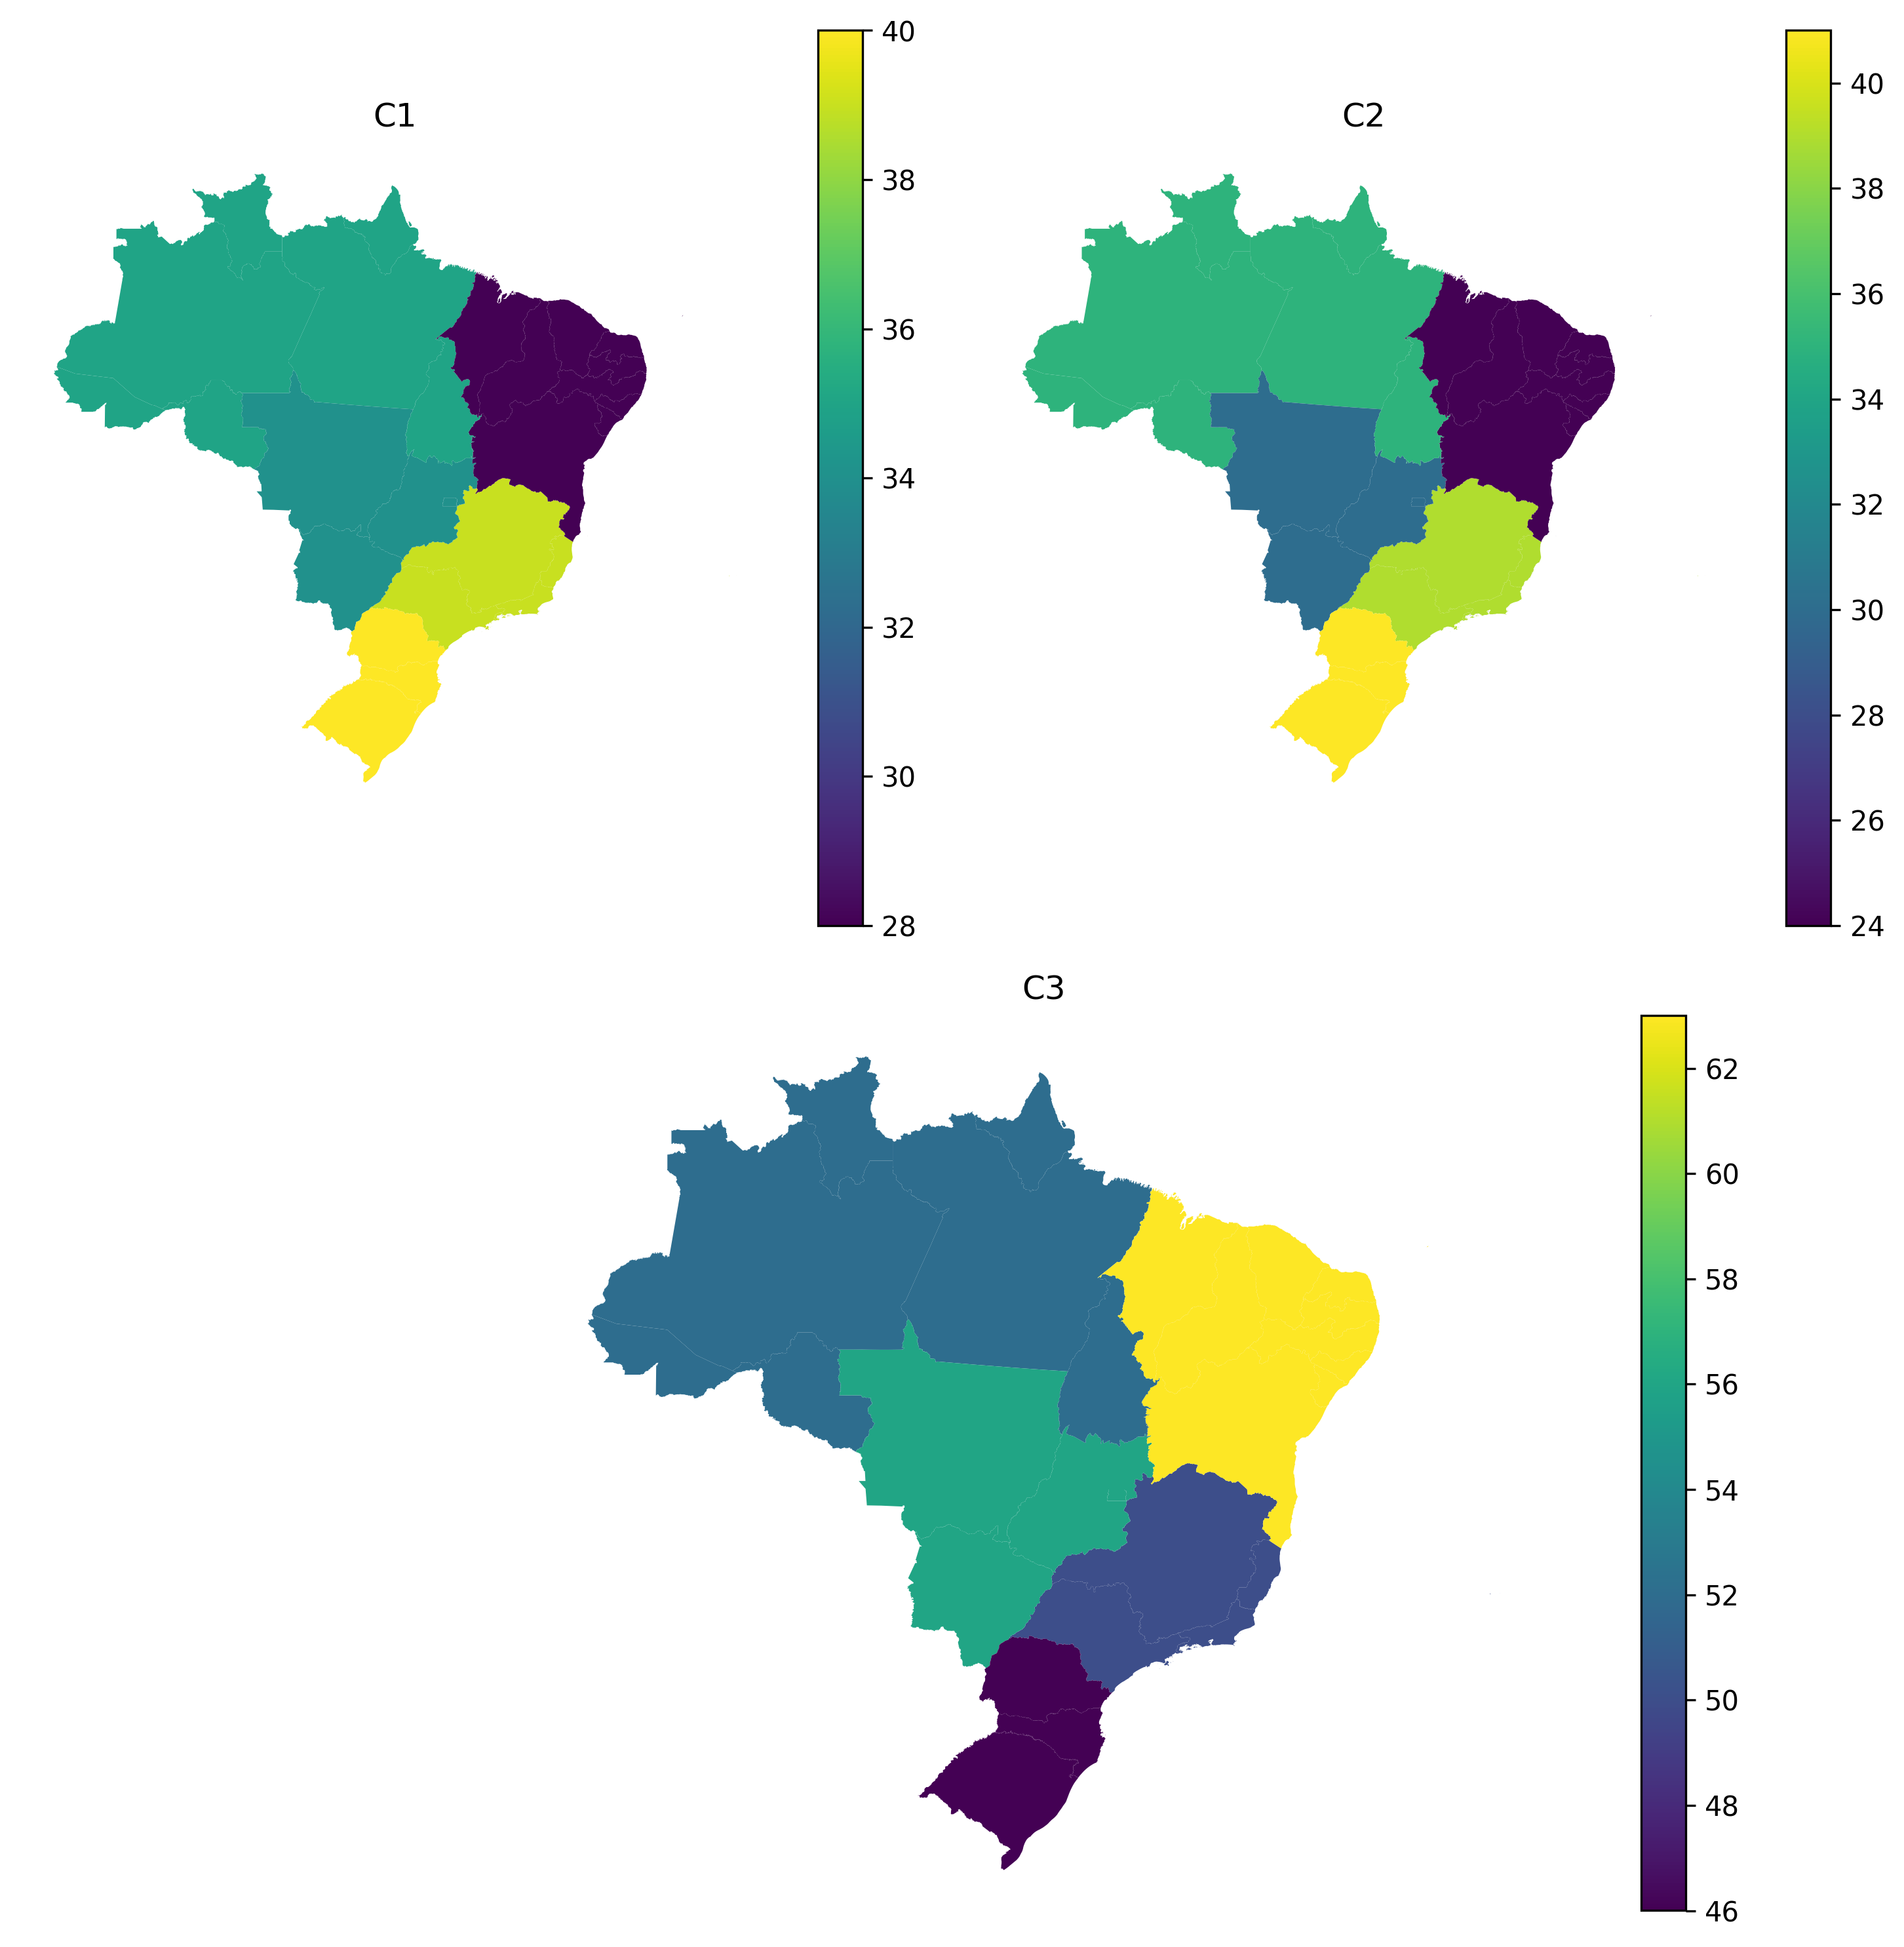
\includegraphics[width=1\linewidth]{figuras/mapa_coropletico_tic_domicilios_2024_g3.png}
	\label{fig:mapa_coropletico_tic_domicilios_2024_g3}
	\footnotesize{Fonte: elaboração própria baseade em \cite{tic_domicilios_2024_g3}.}
\end{figure}

No tocante ao critério G3-1, as regiões Sudeste e Sul foram as regiões em que mais houve procura de informações oferecidas pelo governo, seguidas do Centro-Oeste e Norte, e por fim, pelo Nordeste.

No tocante ao critério G3-2, a região Sul foi a região em que foram realizados alguns serviços públicos, como emitir documentos pela internet, preencher e enviar formulários online ou pagar taxas e impostos pela internet. A região que menos usou serviços públicos foi a Nordeste, superada pelas Centro-Oeste, Norte e Sudeste.

No tocante ao critério G3-3, o Nordeste foi a única região em que a internet não foi utilizada para interagir com as autoridades, seguido do Centro-Oeste e finalmente, o Sudeste e o Sul.

Como foi demonstrado por todas as figuras, nota-se como é notório o uso de governo eletrônico no Brasil. Tal resultado confirma a ideia de \cite{singh2007country}, que argumenta que o uso constante de governo eletrônico justifica sua existência, manutenção e evolução.

\section{Transação do governo eletrônico para o digital no Brasil}

Para \cite{kreuz20184textordfeminine}, vive-se e assiste-se à chegada da 4ª Revolução Industrial, que imprime uma modificação substancial na forma pela qual as pessoas e os diversos sistemas se relacionam. 

Complementa \cite{kreuz20184textordfeminine} que o mundo jurídico e o poder estatal necessitam não apenas se adaptar, mas incorporar as tecnologias ao seu m\textit{modus operandi} como meio de implementar a participação social dos cidadãos no processo decisório. E assim, incorporar os preceitos reais de um constitucionalismo latino-americano.

\cite{kreuz20184textordfeminine} argumenta que o estudo de caso realizado mediante o Governo digital brasileiro fornece algumas respostas. O Brasil vem se adaptando e implementando as TICs nos seus processos de relação com a sociedade. A abertura de dados e transparência cresce a cada ano. 

\cite{kenosi2024industrial} em sua revisão da litaratura, indetificou que sua revião sistemática evidência que o potencial transformativo das tecnologias da Revolução Industrial 4.0 em melhorar os serviços de governo eletronico, focando na democrtização da administração pública vi a transparência melhorada, participação cidadã e entrega de serviços públicos.

No referido contexto, como marco legal da transição de governo eletrônico para digital  no Brasil, a \textbf{Lei do Governo Digital}, em seu artigo 1º, segundo \cite{l14129},  dispõe sobre princípios, regras e instrumentos para o aumento da eficiência da administração pública, especialmente por meio da desburocratização, da inovação, da transformação digital e da participação do cidadão.

Para \cite{do2022governo}, a \text{Lei do Governo Digital}, propondo um modelo de governo digital que inaugure uma nova forma de relacionamento entre a Administração Pública e os destinatários de sua atuação, incorpora ferramentas de modificação na dinâmica tradicional regedora dessas mesmas relações.

Ainda para \cite{do2022governo}, em razão do argumento anterior, promove uma conciliação entre a racionalidade jurídica, que se encontra na regularidade do procedimento e na estabilidade das estruturas formais de organização e atuação, e a racionalidade da gestão, que tem por fonte de legitimidade a eficácia das ações desenvolvidas. 

\cite{do2022governo} elogia a mudança do paradigma legal introduzida pela \text{Lei do Governo Digital} como uma a iniciativa é de ser prestigiada, pois no alinhamento entre racionalidade jurídica e racionalidade da gestão tem-se a tradução de um direito fundamental à boa administração.

Em verdade, ,35 e por isso .

A \textbf{Lei do Governo Digital} nasceu do Projeto de Lei nº 7.843, de 2017. \cite{pl_lgd} cita como motivações para a proposição da inovação legislativa:

\begin{itemize}
    \item As críticas da qualidade ao atendimento do setor público.
    \item A precariedade e a falta de acesso a serviços públicos como fatores determinantes para o grave quadro de exclusão e desigualdade social que sempre marcou a sociedade brasileira. 
    \item  A simplificação das relações entre pessoas,
    sejam elas físicas ou jurídicas, com o poder público, tema essencial para o acesso a direitos básicos e, principalmente, para o desenvolvimento econômico.
    \item O excesso de exigências burocráticas, a baixa informatização, o ainda frágil acesso à informação, a falta de abertura das bases de dados públicos, a ausência de mecanismos de participação e inovação, além da corrupção, são alguns dos problemas que explicam a precariedade e ineficiência dos serviços públicos prestados
    nas três esferas da federação.
\end{itemize}

Nesse sentido, a \textbf{Lei do Governo Digital}, visando melhorar a administração pública, seu artigo 5º, conforme \cite{l14129}, serão utilizadas soluções digitais para a gestão de suas políticas finalísticas e administrativas e para o trâmite de processos administrativos eletrônicos.

Além disso, \textbf{Lei do Governo Digital}, segundo \cite{l14129}, determina sua aplicação às Administrações Direta e Indireta da União Federal e dos demais entes federados, desde que adotem os comandos da lei por meio de atos normativos próprios, vedada a aplicação da lei às empresas públicas e sociedades de economia mista, suas subsidiárias e controladas que não prestem serviço público.

Haja vista \cite{reck2021transformaccao}, o governo digital não se restringe à automação de processos e à disponibilização de serviços públicos on-line, busca avançar para um modelo de administração pública capaz de integrar as TICs a seus processos internos e aos cidadãos, buscando cumprir os papéis essenciais do Estado de forma mais eficiente, bem como restar serviços públicos mais qualificados. 

De forma complementar ao argumento anterior, \cite{lima2023governo}, com as inovações legislativas trazidas pela \textbf{Lei do Governo Digital}, especialmente com o enfoque em um modelo do Governo digital por plataforma, notadamente na esfera federal, a mudança está em sintonia com as mudanças tecnológicas, principalmente impulsionadas pela pandemia da Covid-19, guarda estrita sintonia com a ordem jurídica constitucional vigente e evidencia essa ordem de preocupação normativa da parte do Poder Público.

A maneira como o poder público se relaciona com a sociedade civil, sob a ótica do governo digital, segundo  \cite{lima2023governo}, é via as plataformas de governo digital, pois constituem realizações que buscam a aproximação entre Administração e cidadãos e cidadãs na esfera digital e, adicionalmente, são os meios pelos quais a atuação pública alcança suas finalidades.

Para \cite{de2020governo}, ao longo dos anos, a administração pública no Brasil se estruturou e foi moldada a partir de um amálgama entre uma concepção jurídica formalista, práticas burocráticas e uma generalizada cultura da desconfiança. 

\cite{de2020governo} complementa a ideia anterior citando as diversas faces 
conhecidas do modelo democrático:  

\begin{itemize}
    \item Interpretações e decisões baseadas em conceitos abstratos, ignorando as suas consequências práticas, defesa de ritos e formas como um fim em si mesmo, exigências de regularização desnecessárias.
    \item Um ambiente institucional que incentiva e premia o conservadorismo e a apatia de servidores e gestores públicos.
\end{itemize}

\cite{de2020governo} argumenta que as iniciativas de governo digital - sucessoras do governo eletrônico - pretendem, justamente, transformar a realidade do modelo burocrático inefetivo, eficaz  e ineficiente, mediante a instituição de serviços públicos digitais, que sejam mais simples, céleres e eficientes.

A implementação das iniciativas de governo digital trata-se, segundo \cite{de2020governo}, da construção de um novo paradigma  de administração pública, fundado sobre os princípios da transparência, da inovação e da confiança  segundo os quais o uso das tecnologias digitais pode e deve viabilizar: 

\begin{itemize}
    \item A ampliação do acesso às informações públicas e a simplificação de 
    mecanismos de prestação de contas e de interação entre a administração 
    pública e a sociedade, incluindo a instituição de novos mecanismos de 
    avaliação dos serviços.
    \item A efetiva e constante inovação, mediante a adoção de modelos 
    administrativos e jurídicos flexíveis, a admissibilidade controlada do risco, a relativa tolerância ao erro, o questionamento de práticas vigentes e a criação de incentivos para a experimentação e para a implementação de soluções criativas por parte de gestores públicos.
    \item Com base na arquitetura disponibilizada pelas tecnologias digitais, a constituição de novos modos de produção da confiança, por meio dos quais seja possível a redução de exigências burocráticas, bem como a garantia de maior simplicidade, celeridade, previsibilidade e segurança nas relações entre cidadãos e órgãos e entidades públicos.
\end{itemize}

Relativo ao primeiro tópico, o Brasil sanou o problema citado com a aprovação da Lei nº 12.527, de 2011 - Lei de Acesso à Informação e com a implementação dos portais da transparência do órgãos e Poderes dos Entes Federados.

O segundo tópico foi sanado pelo \textbf{Lei do Governo Digital} pela criação dos laboratórios de inovação. Para \cite{l14129}, laboratório de inovação é um espaço aberto à participação e à colaboração da sociedade para o desenvolvimento de ideias, de ferramentas e de métodos inovadores para a gestão pública, a prestação de serviços públicos e a participação do cidadão no exercício do controle sobre a administração pública.

O último e terceiro tópico foi sanado com a determinação legal de que apenas o CPF, para pessoas físicas, e o CNPJ, para pessoas jurídicas, como a única forma de identificação aceita pela administração pública, haja vista a \textbf{Lei do Governo Digital} (art. 28, \textbf{caput}), conforme exposto por \cite{l14129}: "Art. 28.  Fica estabelecido o número de inscrição no Cadastro de Pessoas Físicas (CPF) ou no Cadastro Nacional da Pessoa Jurídica (CNPJ) como número suficiente para identificação do cidadão ou da pessoa jurídica, conforme o caso, nos bancos de dados de serviços públicos, garantida a gratuidade da inscrição e das alterações nesses cadastros."

Independentemente dos benefícios apresentados pelos argumentos anteriores, considerando \cite{de2020governo} a ideia de que há diversos obstáculos que podem dificultar ou desvirtuar o sentido e os resultados das políticas de governo digital, dentre elas: o risco de digitalização de fachada e se foi realizada sem as devidas salvaguardas técnicas e jurídicas.

No tocante ao risco de digitalização de fachada, segundo \cite{de2020governo}, pode ocorrer a manutenção da lógica burocrática tradicional sob uma roupagem eletrônica, equívoco muitas vezes encontrado na administração pública brasileira. O segundo problema, a incorporação de tecnologias digitais pode gerar externalidades negativas, produzindo novos riscos e incertezas ou, ainda, abusos e violação de direitos.

Outros fatores são citados como barreiras para a implementação das políticas de governo digital, são para \cite{do2022governo}: 

\begin{itemize}
    \item No campo da resistência cultural, o investimento, obrigatoria
    mente, deve ser no treinamento e na formação das lideranças públicas 
    a conduzirem o processo.
    \item Na relação com o controle, as iniciativas associadas 
    ao governo digital devem se pautar, principalmente, pelo sempre pres
    tigiado vetor da transparência
\end{itemize}

No tocante ao primeiro tópico, \cite{do2022governo} afirma que o investimento, obrigatoriamente, deve ser no treinamento e na formação das lideranças públicas 
a conduzirem o processo. Educação digital deve ser a palavra de ordem dentro da Administração, para os seus próprios agentes, e em favor dos destinatários do governo digital. 

Como resultado da educação para mitigar a resistência à digitalização do poder público, segundo \cite{do2022governo}, ampliada a educação digital, o valor inerente ao governo de mesmo cariz resta autoevidente, e com isso a tendência é de mitigação da resistência a partir da perspectiva de constrição fiscal.

No tocante ao segundo e último tópico, \cite{do2022governo} argumenta que na relação com o controle, principalmente, pelo sempre prestigiado vetor da transparência. O problema não está em navegar em mares nunca dantes navegados, mas sim, em não ter clareza quanto às ondas que se possam ter pela frente.